% Options for packages loaded elsewhere
\PassOptionsToPackage{unicode}{hyperref}
\PassOptionsToPackage{hyphens}{url}
%
\documentclass[
]{book}
\usepackage{amsmath,amssymb}
\usepackage{lmodern}
\usepackage{iftex}
\ifPDFTeX
  \usepackage[T1]{fontenc}
  \usepackage[utf8]{inputenc}
  \usepackage{textcomp} % provide euro and other symbols
\else % if luatex or xetex
  \usepackage{unicode-math}
  \defaultfontfeatures{Scale=MatchLowercase}
  \defaultfontfeatures[\rmfamily]{Ligatures=TeX,Scale=1}
\fi
% Use upquote if available, for straight quotes in verbatim environments
\IfFileExists{upquote.sty}{\usepackage{upquote}}{}
\IfFileExists{microtype.sty}{% use microtype if available
  \usepackage[]{microtype}
  \UseMicrotypeSet[protrusion]{basicmath} % disable protrusion for tt fonts
}{}
\makeatletter
\@ifundefined{KOMAClassName}{% if non-KOMA class
  \IfFileExists{parskip.sty}{%
    \usepackage{parskip}
  }{% else
    \setlength{\parindent}{0pt}
    \setlength{\parskip}{6pt plus 2pt minus 1pt}}
}{% if KOMA class
  \KOMAoptions{parskip=half}}
\makeatother
\usepackage{xcolor}
\IfFileExists{xurl.sty}{\usepackage{xurl}}{} % add URL line breaks if available
\IfFileExists{bookmark.sty}{\usepackage{bookmark}}{\usepackage{hyperref}}
\hypersetup{
  pdftitle={Little Kids, Big Adventures Around Knoxville, Tennessee},
  pdfauthor={Katie Rosenberg and Joshua Rosenberg},
  hidelinks,
  pdfcreator={LaTeX via pandoc}}
\urlstyle{same} % disable monospaced font for URLs
\usepackage{longtable,booktabs,array}
\usepackage{calc} % for calculating minipage widths
% Correct order of tables after \paragraph or \subparagraph
\usepackage{etoolbox}
\makeatletter
\patchcmd\longtable{\par}{\if@noskipsec\mbox{}\fi\par}{}{}
\makeatother
% Allow footnotes in longtable head/foot
\IfFileExists{footnotehyper.sty}{\usepackage{footnotehyper}}{\usepackage{footnote}}
\makesavenoteenv{longtable}
\usepackage{graphicx}
\makeatletter
\def\maxwidth{\ifdim\Gin@nat@width>\linewidth\linewidth\else\Gin@nat@width\fi}
\def\maxheight{\ifdim\Gin@nat@height>\textheight\textheight\else\Gin@nat@height\fi}
\makeatother
% Scale images if necessary, so that they will not overflow the page
% margins by default, and it is still possible to overwrite the defaults
% using explicit options in \includegraphics[width, height, ...]{}
\setkeys{Gin}{width=\maxwidth,height=\maxheight,keepaspectratio}
% Set default figure placement to htbp
\makeatletter
\def\fps@figure{htbp}
\makeatother
\setlength{\emergencystretch}{3em} % prevent overfull lines
\providecommand{\tightlist}{%
  \setlength{\itemsep}{0pt}\setlength{\parskip}{0pt}}
\setcounter{secnumdepth}{5}
\usepackage{booktabs}
\usepackage{booktabs}
\usepackage{longtable}
\usepackage{array}
\usepackage{multirow}
\usepackage{wrapfig}
\usepackage{float}
\usepackage{colortbl}
\usepackage{pdflscape}
\usepackage{tabu}
\usepackage{threeparttable}
\usepackage{threeparttablex}
\usepackage[normalem]{ulem}
\usepackage{makecell}
\usepackage{xcolor}
\ifLuaTeX
  \usepackage{selnolig}  % disable illegal ligatures
\fi
\usepackage[]{natbib}
\bibliographystyle{apalike}

\title{Little Kids, Big Adventures Around Knoxville, Tennessee}
\usepackage{etoolbox}
\makeatletter
\providecommand{\subtitle}[1]{% add subtitle to \maketitle
  \apptocmd{\@title}{\par {\large #1 \par}}{}{}
}
\makeatother
\subtitle{Learning About and Experiencing the Cumberland Plateau, Tennessee Valley, and Great Smoky Mountains}
\author{Katie Rosenberg and Joshua Rosenberg}
\date{Last updated: 2022-01-31}

\begin{document}
\maketitle

{
\setcounter{tocdepth}{1}
\tableofcontents
}
\hypertarget{preamble}{%
\chapter*{Preamble}\label{preamble}}
\addcontentsline{toc}{chapter}{Preamble}

\hypertarget{welcome}{%
\section*{Welcome}\label{welcome}}
\addcontentsline{toc}{section}{Welcome}

Welcome to our book! This book is intended to serve as a resource for anyone looking to learn about or experience the outdoors around Knoxville, Tennessee.

Our aim in writing this is primarily to serve as an accessible guide to others looking to learn more about the outdoors around Knoxville. It is written with someone either new to Knoxville or someone who is looking to learn about the outdoors areas around Knoxville. For example, we take care to explain what we mean when we point to locations like the Cumberland Plateau (and how locations like \emph{The Plateau} are different from the Smokies and the area in which Knoxville may be found, the Tennessee Valley.)

It will also have elements that will be of interest to those with more knowledge about and experience exploring the outdoors around Knoxville. For example, we've included detailed trail maps for each location and we include historical and scientific information to add context to the areas we describe.

To sum up the above, this is a book \emph{primarily} but not exclusively for those looking to explore the outdoors around Knoxville, Tennessee who hope to do so with children. No experience with exploring the outdoors, in general, nor with the outdoors around Knoxville, is assumed. We focus on hiking, but mention other activities when relevant. Having established the audience, we next turn to some \emph{other} aspects of the book.

\hypertarget{prologue}{%
\section*{Prologue}\label{prologue}}
\addcontentsline{toc}{section}{Prologue}

We moved to Knoxville from Michigan in 2018. When we moved, we knew about the Smokies - it's hard not to read about them when reading about Knoxville. But, the Smokies are \emph{huge} - and while there is a lot of information about the Smokies available, it can be hard to parse. Are these recommended places also the most busy? Where are the hidden gems - the places locals go? hat's practical to make it to on a day trip from Knoxville? It's too easy to end up on a busy trail (or, much worse, stuck in traffic) in the amazing place that is the Smokies, instead of enjoying one of the most incredible outdoors areas in the world (really!).

We didn't know about much besides the Smokies. We heard a bit about the Urban Wilderness and Ijams, both a few minutes from downtown. At the same time, there seemed to be even more to do, including in the direction away from the Smokies. What is the Obed river? And Big South Fork?

Then, there was the pandemic. Especially with a young child in the early days of the pandemic, there were not many activities to do: even events outdoors (and, early on, even playgrounds!) were closed.

Collectively, the above reasons invited us to start to learn more about the outdoors areas around Knoxville. We started slow - a trip to the part of the Smokies closest to Knoxville, Abrams Creek; a drive out to Obed Wild \& Scenic River on a whim; hearing about Seven Islands Birding State Park within 30 minutes of our house and taking a morning excursion there. The results were good. We liked the places we went.

As we spent more time exploring (and the COVID-19 pandemic did not relent), we explored more, returning to the same places - Abrams Creek in the Smokies, Obed Wild \& Scenic River, Seven Islands State Birding Park - and traveling to new places---places across the Smokies, places nearer to our house in the Tennessee Valley (that includes Knoxville), and places to the other side of the Smokies, on and around what we learned is termed the Cumberland Plateau. We started to make memories as a family and individually - trips around holidays and birthdays for which the weather was just right, we were happy to be together, and we started to feel like we liked this place.

This book is the result of these experiences. It resulted from a lot of \emph{learning about} and \emph{experiencing} the places around Knoxville.

\hypertarget{how-to-use}{%
\section*{How to Use}\label{how-to-use}}
\addcontentsline{toc}{section}{How to Use}

\textbf{First and foremost, please note that this book is a work-in-progress; it is not even at the rough draft stage yet!}

\hypertarget{trails-index}{%
\section*{Trails Index}\label{trails-index}}
\addcontentsline{toc}{section}{Trails Index}

The book is organized around trails in three regions: the Tennessee Valley, Cumberland Plateau, and Smokies. An overview of all of the trails included in the book are below.

Related to trails, a big part of exploring is finding your own tips and tricks and ways to navigate particular places. We highlight some of our tips with this type of call-out.

\begin{rmdtip}
This is a tip.
\end{rmdtip}

\begin{table}
\centering
\begin{tabular}[t]{l|l|l|r|r|r}
\hline
Hike Name & Location & Region & Distance (Shorter Option) & Ascend (Shorter Option) & Max. Elevation (Shorter Option)\\
\hline
Knox/Blount Greenway & Cherokee Farm & The Tennessee Valley & 1.54 & 78 & 859\\
\hline
William Hastie & William Hastie Natural Area & The Tennessee Valley & 0.91 & 59 & 991\\
\hline
Seven Islands Island Loop & Seven Islands State Birding Park & The Tennessee Valley & 2.39 & 191 & 959\\
\hline
Ijams Overlook & Ijams Nature Center & The Tennessee Valley & 1.51 & 181 & 1000\\
\hline
Lakeshore Loop & Lakeshore Park & The Tennessee Valley & 2.33 & 194 & 921\\
\hline
House Mountain Overlook & House Mountain State Natural Area & The Tennessee Valley & 2.50 & 912 & 2031\\
\hline
Songbird Trail & Norris Dam State Park & The Tennessee Valley & 2.41 & 186 & 872\\
\hline
Schoolhouse Gap and Whiteoak Sinks & Great Smoky Mountains National Park & The Smokies and Beyond & 4.61 & 896 & 1869\\
\hline
Abrams Creek & Great Smoky Mountains National Park & The Smokies and Beyond & 5.78 & 991 & 1425\\
\hline
Middle Prong & Great Smoky Mountains National Park & The Smokies and Beyond & 7.73 & 1272 & 3155\\
\hline
Big Creek & Great Smoky Mountains National Park & The Smokies and Beyond & 4.01 & 821 & 2359\\
\hline
Little River Loop & Great Smoky Mountains National Park & The Smokies and Beyond & 5.49 & 996 & 3042\\
\hline
Abrams Falls & Great Smoky Mountains National Park & The Smokies and Beyond & 4.97 & 846 & 1801\\
\hline
Andrews Bald & Great Smoky Mountains National Park & The Smokies and Beyond & 3.57 & 927 & 6307\\
\hline
Cosby Nature Trail & Great Smoky Mountains National Park & The Smokies and Beyond & 0.79 & 124 & 2390\\
\hline
Bandy Creek & Big South Fork National River and Recreation Area & The Cumberland Plateau & 3.67 & 363 & 1601\\
\hline
Emory Falls & Frozen Head State Park & The Cumberland Plateau & 2.43 & 480 & 2036\\
\hline
Honey Creek & Big South Fork National River and Recreation Area & The Cumberland Plateau & 4.40 & 962 & 1587\\
\hline
Twin Arches Loop & Twin Arches State Recreation Area & The Cumberland Plateau & 1.15 & 297 & 1574\\
\hline
Obed Point & Obed Wild \& Scenic River & The Cumberland Plateau & 3.60 & 761 & 1361\\
\hline
\end{tabular}
\end{table}

\hypertarget{science-related-elements}{%
\section*{Science-Related Elements}\label{science-related-elements}}
\addcontentsline{toc}{section}{Science-Related Elements}

We use the following call-out for scientific tid-bits: those related to living and non-living aspects of the environment that have been studied scientifically, such as the names of plants and animals or the types of rock underfoot.

\begin{rmdscience}
This is for science-related call-outs.
\end{rmdscience}

The following species and topics are discussed:

\begin{table}
\centering
\begin{tabular}[t]{l|l}
\hline
Name & Type\\
\hline
Eastern Hemlock & Tree\\
\hline
Rosebay Rhododendron & Tree\\
\hline
Mountain Laurel & Tree\\
\hline
Tulip Poplar & Tree\\
\hline
Frasier Fir & Tree\\
\hline
Red Spruce & Tree\\
\hline
Brook Trout & Fish\\
\hline
Black Bear & Mammal\\
\hline
Coyote & Mammal\\
\hline
White-tailed Deer & Mammal\\
\hline
Trillium & Wildflower\\
\hline
Blue Phlox & Wildflower\\
\hline
Thyme-Leaved Bluets & Wildflower\\
\hline
Trout-Lily & Wildflower\\
\hline
Downy Woodpecker & Bird\\
\hline
Eastern Screech Owl & Bird\\
\hline
Carolina Chickadee & Bird\\
\hline
Eastern Box Turtle & Reptile\\
\hline
Northern Copperhead & Reptile\\
\hline
Timber Rattlesnake & Reptile\\
\hline
Eastern Hellbender & Amphibian\\
\hline
Blue Ridge Two-Lined Salamander & Amphibian\\
\hline
Jordans Red Cheek & Amphibian\\
\hline
Tardigrade & Micro-Animal\\
\hline
Anakeesta Formation & Geological\\
\hline
Thunderhead Formation & Geological\\
\hline
Sandstone & Geological\\
\hline
\end{tabular}
\end{table}

\hypertarget{history-related-elements}{%
\section*{History-Related Elements}\label{history-related-elements}}
\addcontentsline{toc}{section}{History-Related Elements}

Though we have more expertise in science, we call-out history-related elements of the areas in this book with the following:

\begin{rmdhistory}
This is for human history-related call-outs.
\end{rmdhistory}

The following historical topics and events are discussed:

\begin{table}
\centering
\begin{tabular}[t]{l|l}
\hline
Name & Type\\
\hline
Elkmont Cabins & Recreation\\
\hline
Little River Lumber Company & Industry\\
\hline
Champion Lumber Company & Industry\\
\hline
Tsali and the Cherokee & Human History\\
\hline
Norris Dam & Industry\\
\hline
Kelly Farm & Agriculture\\
\hline
Brushy Mountain State Penetentiary Escape and Capture & Event\\
\hline
Angel Falls & Event\\
\hline
Roan Mountain & Human History\\
\hline
Ijams Quarry & Industry\\
\hline
Black Balsam Fire & Industry\\
\hline
Moonshining & Human History\\
\hline
Abram & Human History\\
\hline
Cade's Cover & Agriculture\\
\hline
Cumberland Trail & Human History\\
\hline
Appalachian Trail & Human History\\
\hline
\end{tabular}
\end{table}

\hypertarget{onward}{%
\section*{Onward!}\label{onward}}
\addcontentsline{toc}{section}{Onward!}

If you're ready to start to look at trails head straight to sections two, three, or four, about trails in the Tennessee Valley, on the Cumberland Plateau, and in and around the Smokies. If you would like a bit more background, we recommend you head first to the next section on getting started.

\hypertarget{part-get-started}{%
\part{Get Started}\label{part-get-started}}

This section provides information on getting started, including considering the climate and weather, what gear to bring, and planning a trip.

\hypertarget{climate-and-weather}{%
\chapter{Climate and Weather}\label{climate-and-weather}}

\hypertarget{weather}{%
\section{Weather}\label{weather}}

Many guides describe the Tennessee weather in a way like the following:

\begin{quote}
In East Tennessee, there are four seasons of weather, including a hot, humid summer, and a cold winter, with temperatures regularly dipping below freezing. Spring and fall bring mild weather, with a lot of variation, especially around the shoulder months of March-April and October-November.
\end{quote}

This is mostly true, but it fails to capture what it's \emph{like} to live in this area. We moved from Michigan---and Michigan is certainly a place in which there are four seasons. Indeed, it sometimes feels like the winter is the longest season in Michigan. That's not the case in Tennessee as the \emph{balance} between the seasons is different and this has profound impacts.

We'll try to summarize the \emph{experience} of each of the seasons in East Tennessee and how the progression of a typical year may unfold.

\hypertarget{spring}{%
\subsection{Spring}\label{spring}}

\hypertarget{summer}{%
\subsection{Summer}\label{summer}}

\hypertarget{fall}{%
\subsection{Fall}\label{fall}}

\hypertarget{winter}{%
\subsection{Winter}\label{winter}}

\hypertarget{getting-started}{%
\chapter{Getting started}\label{getting-started}}

\hypertarget{gear}{%
\section{Gear}\label{gear}}

`Good' gear is at once over-rated and under-rated. Allow us to explain.

\hypertarget{fitness}{%
\section{Fitness}\label{fitness}}

Start small. Know your limits, have a bail out.

\hypertarget{weather-1}{%
\section{Weather}\label{weather-1}}

Many guides describe the Tennessee weather in a way like the following:

\begin{quote}
In East Tennessee, there are four seasons of weather, including a hot, humid summer, and a cold winter, with temperatures regularly dipping below freezing. Spring and fall bring mild weather, with a lot of variation, especially around the shoulder months of March-April and October-November.
\end{quote}

This is mostly true, but it fails to capture what it's \emph{like} to live in this area. We moved from Michigan---and Michigan is certainly a place in which there are four seasons. Indeed, it sometimes feels like the winter is the longest season in Michigan. That's not the case in Tennessee as the \emph{balance} between the seasons is different and this has profound impacts.

We'll try to summarize the \emph{experience} of each of the seasons in East Tennessee and how the progression of a typical year may unfold.

\hypertarget{spring-1}{%
\subsection{Spring}\label{spring-1}}

\hypertarget{summer-1}{%
\subsection{Summer}\label{summer-1}}

\hypertarget{fall-1}{%
\subsection{Fall}\label{fall-1}}

\hypertarget{winter-1}{%
\subsection{Winter}\label{winter-1}}

\hypertarget{safety}{%
\section{Safety}\label{safety}}

A question that many ask about the Smokies, particularly, but also hiking, generally, has to do with safety concerning a very specific concern: bears. \href{https://www.nps.gov/grsm/learn/nature/black-bears.htm}{There are black bears in the Smokies}: around 1,500 of them.

Moreover, \href{https://trace.tennessee.edu/cgi/viewcontent.cgi?article=7040\&context=utk_gradthes}{there are black bears in the Big South Fork area} of the Cumberland Plateau: The latest estimates suggest that a population of around one dozen bears that were introduced in the late 1990s are doing very well and now comprise a population of nearly 1,000 bears.

Given these numbers of bears and the number of visitors to both parks - \href{https://www.nps.gov/grsm/learn/news/park-experiences-more-than-12-million-visits-in-2020.htm}{more than 12M to the Smokies in 2020 alone}, the number of people who are harmed by bears can be instructive.

\textless\textgreater{} \href{https://outforia.com/danger-parks/\#all-data}{There is data} on the number of people killed in the Smokies. These data provide an important context for a discussion of safety (note, we'll also discuss safety-related issues that don't have to do with death). From 2010-2020, the National Park Service recorded 92 deaths. 42 were from automobile or other transportation-related accidents. 15 were medical/natural deaths. Six were drownings, three were falls, two were poisoning, and 10 were either ``environmental'' or in the other category.

Denominator {[}\url{https://www.psblaw.com/nevada/deaths-in-us-national-parks/}{]}

The park has seen, on average, more than 10M visitors/year from the 2010-2020 period. In the entire history of the park, \href{https://www.knoxnews.com/story/news/local/2020/09/14/great-smokies-rangers-identify-man-found-dead-park-black-bear-scavenging-his-remains/5793471002/}{there have been around six bear attacks} and there have been two deaths from those attacks (in 2000 and 2020). Considering deaths in the last decade, this suggests that bear attacks are exceedingly rare---on the order of one in one hundred million.

Something a lot of people mention about the Smokies is the prevalence of bears. From what I can tell, there have been 6-7 bear attacks in the history of the park and two deaths (2000 \& 2020) from them. Those are bad, but the park received \textasciitilde100M visitors from 2010-2019 alone. This suggests that the risk of dying from a bear attack is around in 100M. The risk of being attacked is somewhere around 1 in 30-60M (as it's somewhat unclear when the documented attacks occurred).

\hypertarget{where-to-begin}{%
\section{Where to begin}\label{where-to-begin}}

Conveient

\hypertarget{gear-1}{%
\chapter{Gear}\label{gear-1}}

\hypertarget{planning}{%
\chapter{Planning}\label{planning}}

\hypertarget{science-primer}{%
\chapter{Science Primer}\label{science-primer}}

\hypertarget{history-primer}{%
\chapter{History Primer}\label{history-primer}}

\hypertarget{introduction-to-the-three-regions}{%
\chapter{Introduction to the Three Regions}\label{introduction-to-the-three-regions}}

\hypertarget{the-tennessee-valley}{%
\section{The Tennessee Valley}\label{the-tennessee-valley}}

\hypertarget{the-cumberland-plateau}{%
\section{The Cumberland Plateau}\label{the-cumberland-plateau}}

I taught at a high school (and went to college) in North Carolina and the drive from North Carolina to
my family in Michigan usually took me through the highway that winds down from around Asheville, past Candler,
and through the heart of the outhern Appalachian mountains. The Appalachian Trail crosses the highway - I-40 -
and at different points along the drive one is between a few and five or so miles from the Smokies. The drive is
often a bit wild; \href{https://www.knoxnews.com/picture-gallery/news/2019/07/17/historic-photos-interstate-40-biggest-rockslides/1656940001/}{rock slides very regularly close the highway, sometimes for weeks}.

At the same time, when moving to Knoxville, I am not sure I could have said what or where the \href{https://en.wikipedia.org/wiki/Cumberland_Plateau}{Cumberland Plateau} is. This sounds absolutely banal, but I believe the key
to initially understanding the area is that it's a plateau--and that makes it distinct from the mountains. Also,
it's different from Michigan.

Here's a picture from this past weekend at \href{https://www.nps.gov/biso/index.htm}{Big South Fork}:

\begin{figure}
\centering
\includegraphics{img/pickett-arch-rock-2.jpeg}
\caption{twin arches in big south fork}
\end{figure}

Ostensibly, one of the \href{https://www.tn.gov/environment/program-areas/na-natural-areas/natural-areas-east-region/east-region-/na-na-twin-arches.html}{Twin Arches} is the largest ock arch in the Eastern United States and one of the largest in the world. I think being a part of the Cumberland Plateau - being close to the Southern Appalachian and Smoky moutains - they slip beneath peoples' radar. There seems to be a near-constant conservation effort, with more \href{https://www.knoxnews.com/story/news/2021/09/23/tennessee-skinner-mountain-cumberland-plateau-now-protected/8417864002/}{land being purchased to be public}. Taking the acreage of Big South Fork National (part of the National Park system; \textasciitilde125,000) and the Cumberland Trail (\textasciitilde35,000), Fall Creek Falls (25,000), Frozen Head (\textasciitilde25,000), South Cumberland (\textasciitilde25,000), and Pickett (20,000) State Parks alone (there are other public lands), this area is around half of the size of the Smokies (\textasciitilde500,000 acres).

This is all to say, I have an interest in spending more time in this area and to try to understand it a bit better.

\hypertarget{the-smokies}{%
\section{The Smokies}\label{the-smokies}}

The Smokies can be a bit hard to get one's head around at first.

It can be hard to get one's head around the Smokies for several reasons:

\begin{itemize}
\tightlist
\item
  Their size: \href{https://www.nps.gov/grsm/learn/nature/index.htm}{more than 800 square miles}
\item
  Their location: split roughly between Tennessee and North Carolina, there are many ways to access the park, and there isn't a \emph{primary} or \emph{best} way to do so
\item
  Their variation in altitude: \href{https://www.nps.gov/grsm/learn/nature/mountains.htm}{Abrams Creek---the trailhead nearest to Knoxville---is roughly 850 feet above sea level, whereas Clingman's Dome is roughly 6,650 feet above sea level}
\item
  Their biodiversity: \href{https://www.nps.gov/grsm/learn/nature/index.htm}{it may be the most biodiverse National Park}
\item
  Their human history: thousands of people of European ancestry lived in what is now the National Park up until as recently as 1934 (when the park was established); before people of European ancestry lived there, thousands of people of Cherokee ancestry lived there; these histories remain alive and present within the park
\end{itemize}

I think these reasons are important in general and in a bit of an abstract sense, but they also have a more personal angle: The Smokies are hard to \emph{experience} for each of these and other reasons, too. They appear and are different in different seasons. They are very different when experienced when walking than when driving in a car. They are different when it's rainy and when it's not. And, they are different alone, with family, with friends, and with a child.

\hypertarget{a-bit-on-my-understanding-of-the-smokies}{%
\subsection{A bit on my understanding of the Smokies}\label{a-bit-on-my-understanding-of-the-smokies}}

When my wife and I first decided to move to Knoxville, I began trying to understand the Smokies, and since then I've read a lot of books and spent a lot of time there. I don't think I can adequately summarize the Smokies, but I can begin to convey my understanding.

The Smokies are a timeless place, at once welcoming and severe. When I drive to the Smokies, I feel like I'm entering into a special place. That special feeling is amplified by the good memories I've had there---with my family and friends and on my own.

I value living by the Smokies a lot. This is a function of a lot of things coming together: stopping refereeing soccer, something I'd done for around 12 years up to that point, soon after we moved to Knoxville, the pandemic, which prevented many other activities from happening, and a live for doing things outdoors that motivated me to study biology and enter teaching to begin.

I'll describe just one trip to try to work to summarize my understanding of the Smokies.

In May, 2020, my wife and little one and I hiked the beginning of the Bote Mountain and West Prong trails to the location of Backcountry site \#18. It was one of our first times heading out after the pandemic began, and it was a moderately difficult hike - around three miles, but with nearly 1,000 feet of climbing. When we arrived at the site---where two creeks meet and are crossed by a log bridge---there were butterflies everywhere, which the little was overjoyed about.

This was one trip, and it was probably one that we planned on a whim, picking the trail based on what was within an hour's drive. That's what made it special; there wasn't anything particularly distinctive about that trail, hike, or day (except for the butterflies, which were pretty neat), and both this absence of distinctiveness coupled with a sense of someting special has nearly always been the case for the time I've spent in the Smokies.

So, as a bit of a thesis, it's hard to understand the Smokies: they're too large, varied, and rich. But, it is possible to experience the Smokies, and doing so doesn't require making it to Mt. LeConte or Abrams Falls or Clingman's Dome (though each of those are pretty great). One can perhaps have just as positive of an experience as at those (sometimes busy) sites off trails or at picnic areas in the Big Creek, Cosby, and Tremont areas.

\hypertarget{part-the-tennessee-valley}{%
\part{The Tennessee Valley}\label{part-the-tennessee-valley}}

\hypertarget{seven-islands-island-loop}{%
\chapter{Seven Islands Island Loop}\label{seven-islands-island-loop}}

\hypertarget{trail-information}{%
\section{Trail Information}\label{trail-information}}

\hypertarget{ratings}{%
\subsection{Ratings}\label{ratings}}

\begin{tabular}{l|r|r|r|r}
\hline
Hike Name & Beauty & Accessibility & Amenities & Challenge\\
\hline
Seven Islands Island Loop & 5 & 4 & 4 & 2\\
\hline
\end{tabular}

\hypertarget{basic-characteristics}{%
\subsection{Basic Characteristics}\label{basic-characteristics}}

Location: Seven Islands State Birding Park\\
Region: The Tennessee Valley\\
Distance: 2.39 (mi.)\\
Elevation (Ascend): 191 (ft.)\\
Max. Elevation: 959 (ft.)

\hypertarget{overview}{%
\section{Overview}\label{overview}}

\hypertarget{map}{%
\section{Map}\label{map}}

\begin{figure}
\includegraphics[width=39.64in]{/Users/joshuarosenberg/little-kids-big-adventures/output/seven-islands-loop-map} \caption{Seven Islands Loop Trail Map}\label{fig:unnamed-chunk-9}
\end{figure}

\hypertarget{trail-description}{%
\section{Trail Description}\label{trail-description}}

\hypertarget{nearby}{%
\section{Nearby}\label{nearby}}

\hypertarget{ijams-quarry-overlook}{%
\chapter{Ijams Quarry Overlook}\label{ijams-quarry-overlook}}

\hypertarget{trail-information-1}{%
\section{Trail Information}\label{trail-information-1}}

\begin{tabular}{l|r|r|r|r}
\hline
Hike Name & Beauty & Accessibility & Amenities & Challenge\\
\hline
Ijams Overlook & 3 & 5 & 5 & 2\\
\hline
\end{tabular}

\hypertarget{basic-characteristics-1}{%
\subsection{Basic Characteristics}\label{basic-characteristics-1}}

Location: Ijams Nature Center\\
Region: The Tennessee Valley\\
Distance: 1.51 (mi.)\\
Elevation (Ascend): 181 (ft.)\\
Max. Elevation: 1000 (ft.)

\hypertarget{overview-1}{%
\section{Overview}\label{overview-1}}

\hypertarget{map-1}{%
\section{Map}\label{map-1}}

\begin{figure}
\includegraphics[width=39.64in]{/Users/joshuarosenberg/little-kids-big-adventures/output/ijams-crag-map} \caption{Seven Islands Loop Trail Map}\label{fig:unnamed-chunk-11}
\end{figure}

\hypertarget{trail-description-1}{%
\section{Trail Description}\label{trail-description-1}}

\hypertarget{nearby-1}{%
\section{Nearby}\label{nearby-1}}

\hypertarget{william-hastie}{%
\chapter{William Hastie}\label{william-hastie}}

\hypertarget{trail-information-2}{%
\section{Trail Information}\label{trail-information-2}}

\begin{tabular}{l|r|r|r|r}
\hline
Hike Name & Beauty & Accessibility & Amenities & Challenge\\
\hline
William Hastie & 3 & 4 & 2 & 1\\
\hline
\end{tabular}

\hypertarget{basic-characteristics-2}{%
\subsection{Basic Characteristics}\label{basic-characteristics-2}}

Location: William Hastie Natural Area\\
Region: The Tennessee Valley\\
Distance: 0.91 (mi.)\\
Elevation (Ascend): 59 (ft.)\\
Max. Elevation: 991 (ft.)

\hypertarget{overview-2}{%
\section{Overview}\label{overview-2}}

\hypertarget{map-2}{%
\section{Map}\label{map-2}}

\begin{figure}
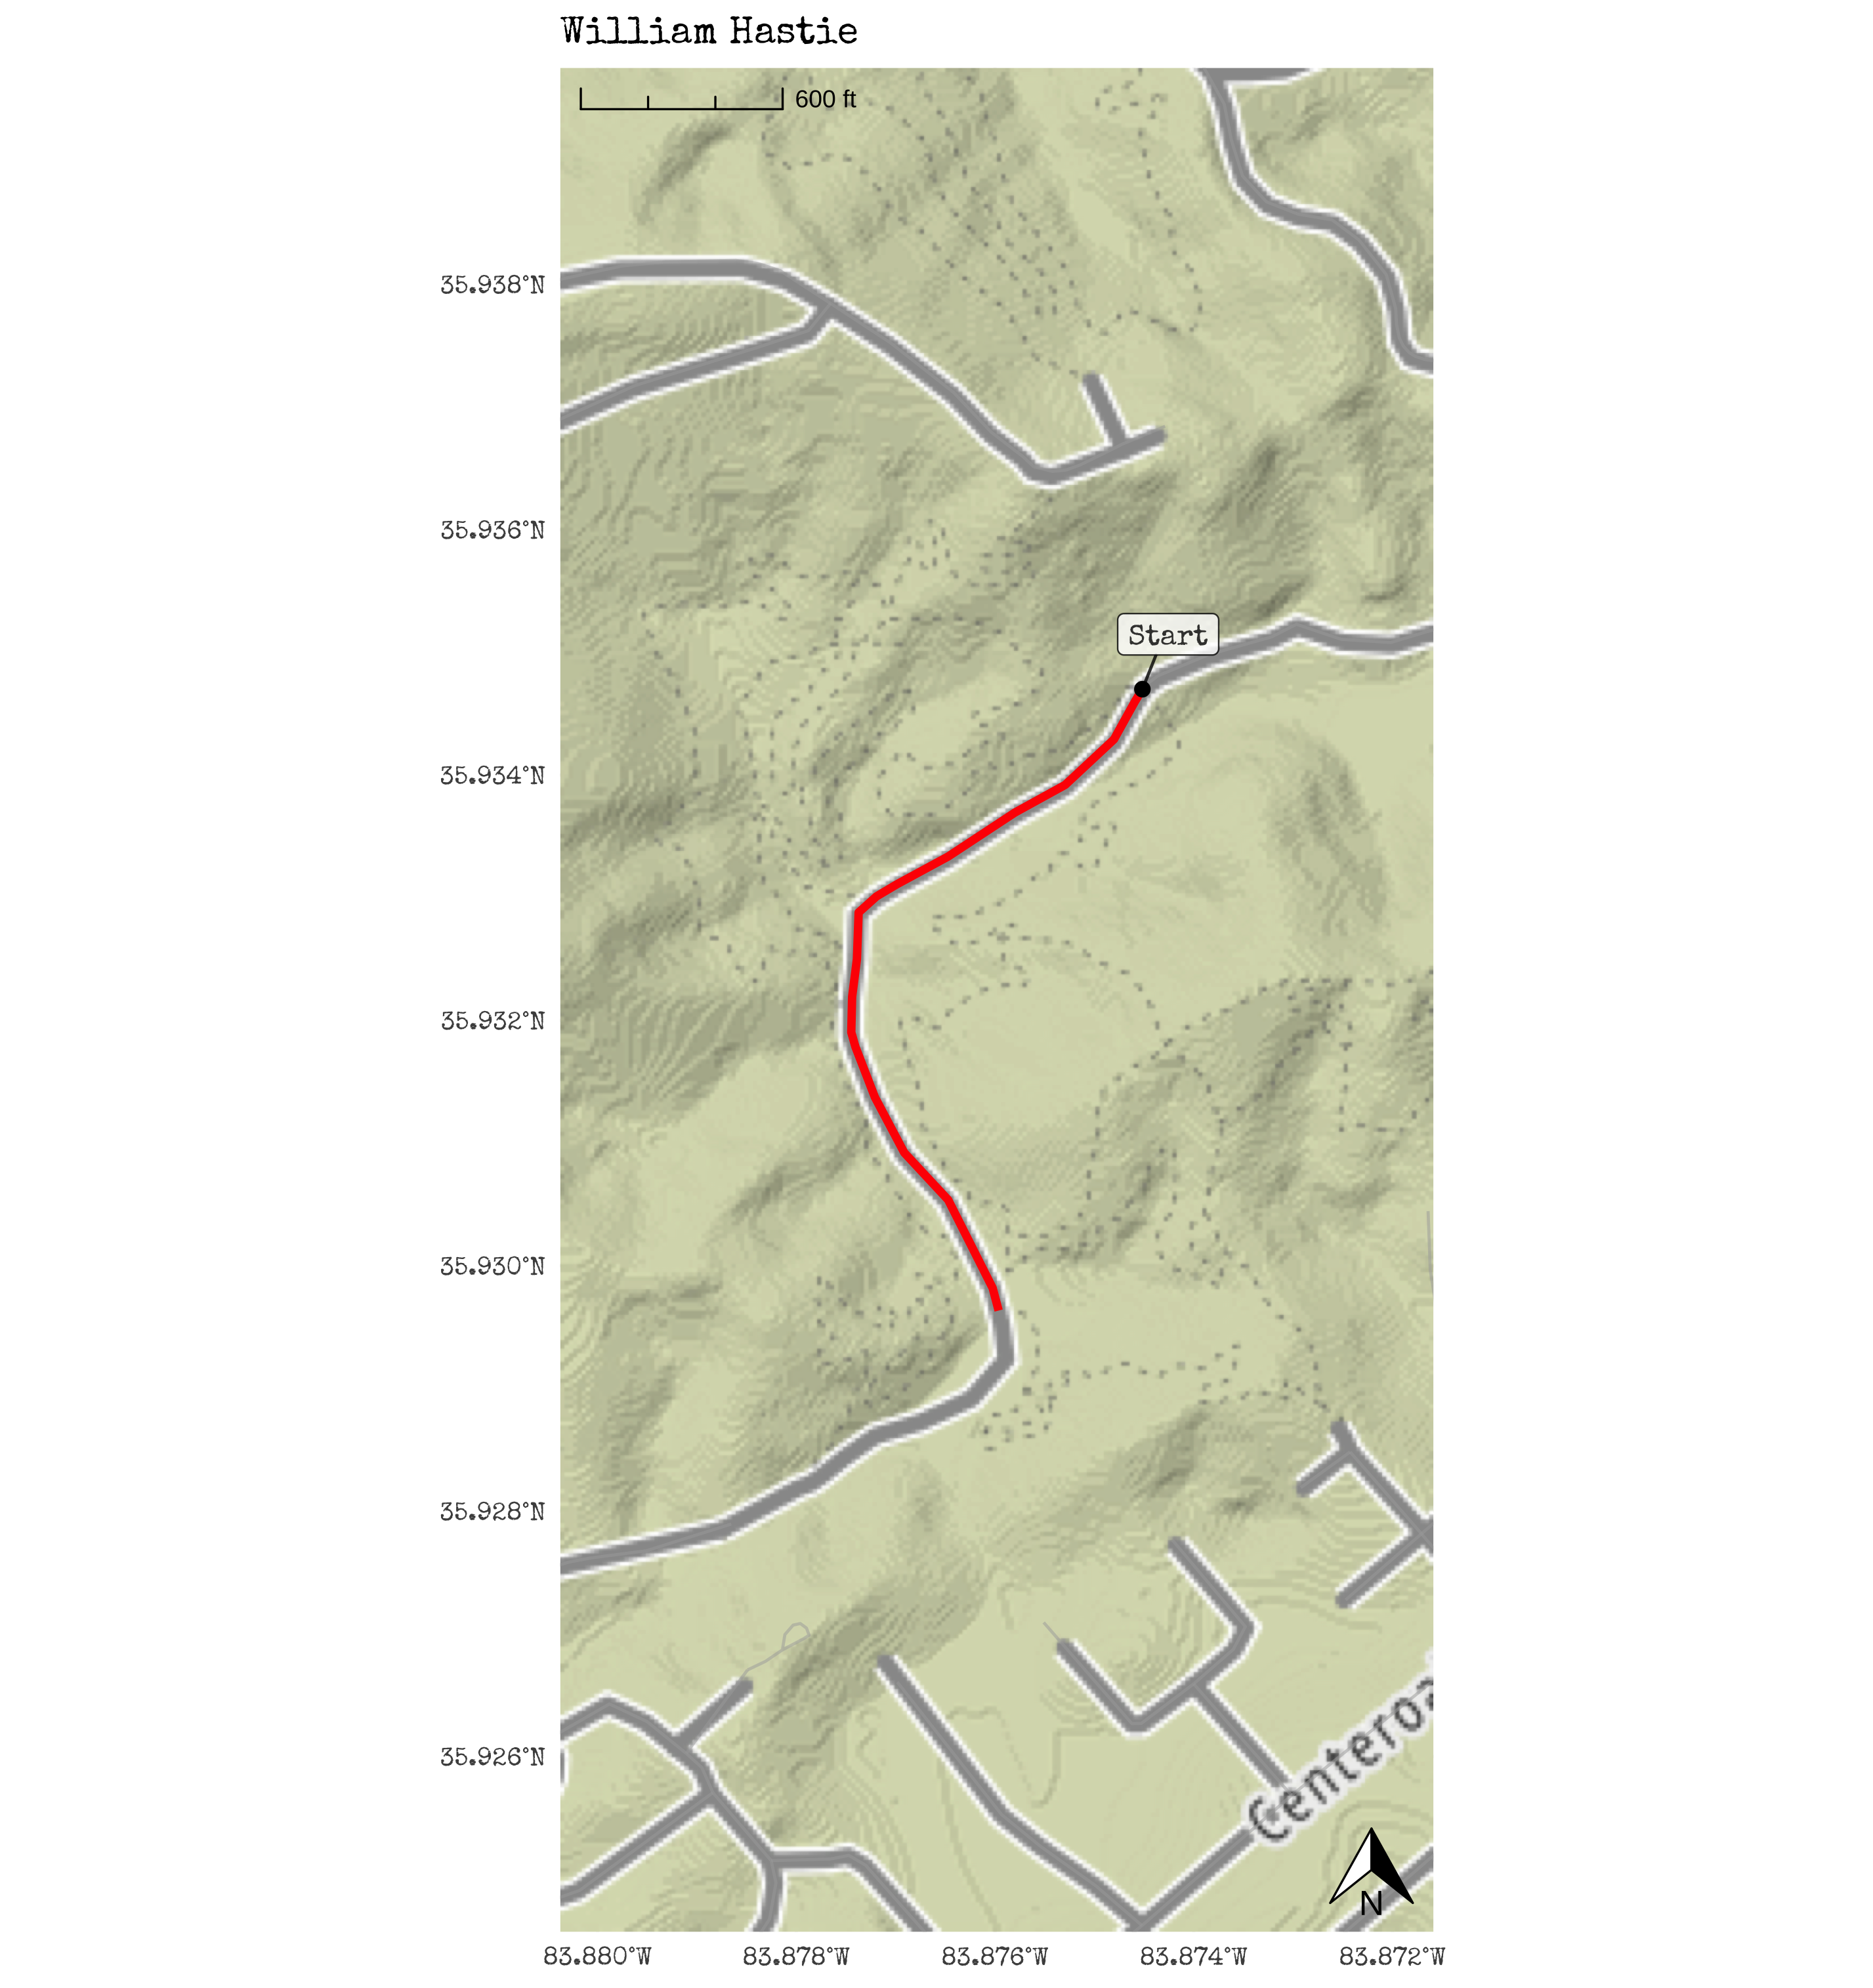
\includegraphics[width=39.64in]{/Users/joshuarosenberg/little-kids-big-adventures/output/william-hastie-map} \caption{Seven Islands Loop Trail Map}\label{fig:unnamed-chunk-13}
\end{figure}

\hypertarget{trail-description-2}{%
\section{Trail Description}\label{trail-description-2}}

\hypertarget{nearby-2}{%
\section{Nearby}\label{nearby-2}}

\hypertarget{knoxblount-greenway}{%
\chapter{Knox/Blount Greenway}\label{knoxblount-greenway}}

\hypertarget{trail-information-3}{%
\section{Trail Information}\label{trail-information-3}}

\begin{tabular}{l|r|r|r|r}
\hline
Hike Name & Beauty & Accessibility & Amenities & Challenge\\
\hline
Knox/Blount Greenway & 2 & 5 & 2 & 1\\
\hline
\end{tabular}

\hypertarget{basic-characteristics-3}{%
\subsection{Basic Characteristics}\label{basic-characteristics-3}}

Location: Cherokee Farm\\
Region: The Tennessee Valley\\
Distance: 1.54 (mi.)\\
Elevation (Ascend): 78 (ft.)\\
Max. Elevation: 859 (ft.)

\hypertarget{overview-3}{%
\section{Overview}\label{overview-3}}

\hypertarget{map-3}{%
\section{Map}\label{map-3}}

\begin{figure}
\includegraphics[width=39.64in]{/Users/joshuarosenberg/little-kids-big-adventures/output/knoxblount-greenway-map} \caption{Seven Islands Loop Trail Map}\label{fig:unnamed-chunk-15}
\end{figure}

\hypertarget{trail-description-3}{%
\section{Trail Description}\label{trail-description-3}}

\hypertarget{nearby-3}{%
\section{Nearby}\label{nearby-3}}

\hypertarget{lakeshore-loop}{%
\chapter{Lakeshore Loop}\label{lakeshore-loop}}

\hypertarget{trail-information-4}{%
\section{Trail Information}\label{trail-information-4}}

\begin{tabular}{l|r|r|r|r}
\hline
Hike Name & Beauty & Accessibility & Amenities & Challenge\\
\hline
Lakeshore Loop & 3 & 4 & 4 & 2\\
\hline
\end{tabular}

\hypertarget{basic-characteristics-4}{%
\subsection{Basic Characteristics}\label{basic-characteristics-4}}

Location: Lakeshore Park\\
Region: The Tennessee Valley\\
Distance: 2.33 (mi.)\\
Elevation (Ascend): 194 (ft.)\\
Max. Elevation: 921 (ft.)

\hypertarget{overview-4}{%
\section{Overview}\label{overview-4}}

\hypertarget{map-4}{%
\section{Map}\label{map-4}}

\begin{figure}
\includegraphics[width=39.64in]{/Users/joshuarosenberg/little-kids-big-adventures/output/lakeshore-loop-map} \caption{Seven Islands Loop Trail Map}\label{fig:unnamed-chunk-17}
\end{figure}

\hypertarget{trail-description-4}{%
\section{Trail Description}\label{trail-description-4}}

\hypertarget{nearby-4}{%
\section{Nearby}\label{nearby-4}}

\hypertarget{house-mountain-overlook}{%
\chapter{House Mountain Overlook}\label{house-mountain-overlook}}

\hypertarget{trail-information-5}{%
\section{Trail Information}\label{trail-information-5}}

\begin{tabular}{l|r|r|r|r}
\hline
Hike Name & Beauty & Accessibility & Amenities & Challenge\\
\hline
House Mountain Overlook & NA & 4 & 1 & 4\\
\hline
\end{tabular}

\hypertarget{basic-characteristics-5}{%
\subsection{Basic Characteristics}\label{basic-characteristics-5}}

Location: House Mountain State Natural Area\\
Region: The Tennessee Valley\\
Distance: 2.5 (mi.)\\
Elevation (Ascend): 912 (ft.)\\
Max. Elevation: 2031 (ft.)

\hypertarget{overview-5}{%
\section{Overview}\label{overview-5}}

\hypertarget{map-5}{%
\section{Map}\label{map-5}}

\begin{figure}
\includegraphics[width=39.64in]{/Users/joshuarosenberg/little-kids-big-adventures/output/house-mountain-overlook-map} \caption{Seven Islands Loop Trail Map}\label{fig:unnamed-chunk-19}
\end{figure}

\hypertarget{trail-description-5}{%
\section{Trail Description}\label{trail-description-5}}

\hypertarget{nearby-5}{%
\section{Nearby}\label{nearby-5}}

\hypertarget{part-the-cumberland-plateau}{%
\part{The Cumberland Plateau}\label{part-the-cumberland-plateau}}

\hypertarget{songbird-loop-norris-dam}{%
\chapter{Songbird Loop (Norris Dam)}\label{songbird-loop-norris-dam}}

\hypertarget{trail-information-6}{%
\section{Trail Information}\label{trail-information-6}}

\hypertarget{ratings-1}{%
\subsection{Ratings}\label{ratings-1}}

\begin{tabular}{l|r|r|r|r}
\hline
Hike Name & Beauty & Accessibility & Amenities & Challenge\\
\hline
Songbird Trail & 3 & 4 & 4 & 2\\
\hline
\end{tabular}

\hypertarget{basic-characteristics-6}{%
\subsection{Basic Characteristics}\label{basic-characteristics-6}}

Location: Norris Dam State Park\\
Region: The Tennessee Valley\\
Distance: 2.41 (mi.)\\
Elevation (Ascend): 186 (ft.)\\
Max. Elevation: 872 (ft.)

\hypertarget{overview-6}{%
\section{Overview}\label{overview-6}}

\hypertarget{map-6}{%
\section{Map}\label{map-6}}

\begin{figure}
\includegraphics[width=39.64in]{/Users/joshuarosenberg/little-kids-big-adventures/output/songbird-loop-map} \caption{Seven Islands Loop Trail Map}\label{fig:unnamed-chunk-21}
\end{figure}

\hypertarget{trail-description-6}{%
\section{Trail Description}\label{trail-description-6}}

\hypertarget{nearby-6}{%
\section{Nearby}\label{nearby-6}}

\hypertarget{obed-point-trail}{%
\chapter{Obed Point Trail}\label{obed-point-trail}}

\hypertarget{trail-information-7}{%
\section{Trail Information}\label{trail-information-7}}

\hypertarget{ratings-2}{%
\subsection{Ratings}\label{ratings-2}}

\begin{tabular}{l|r|r|r|r}
\hline
Hike Name & Beauty & Accessibility & Amenities & Challenge\\
\hline
Obed Point & 5 & 3 & 3 & 4\\
\hline
\end{tabular}

\hypertarget{basic-characteristics-7}{%
\subsection{Basic Characteristics}\label{basic-characteristics-7}}

Location: Obed Wild \& Scenic River\\
Region: The Cumberland Plateau\\
Distance: 3.6 (mi.)\\
Elevation (Ascend): 761 (ft.)\\
Max. Elevation: 1361 (ft.)

\hypertarget{overview-7}{%
\section{Overview}\label{overview-7}}

\hypertarget{map-7}{%
\section{Map}\label{map-7}}

\begin{figure}
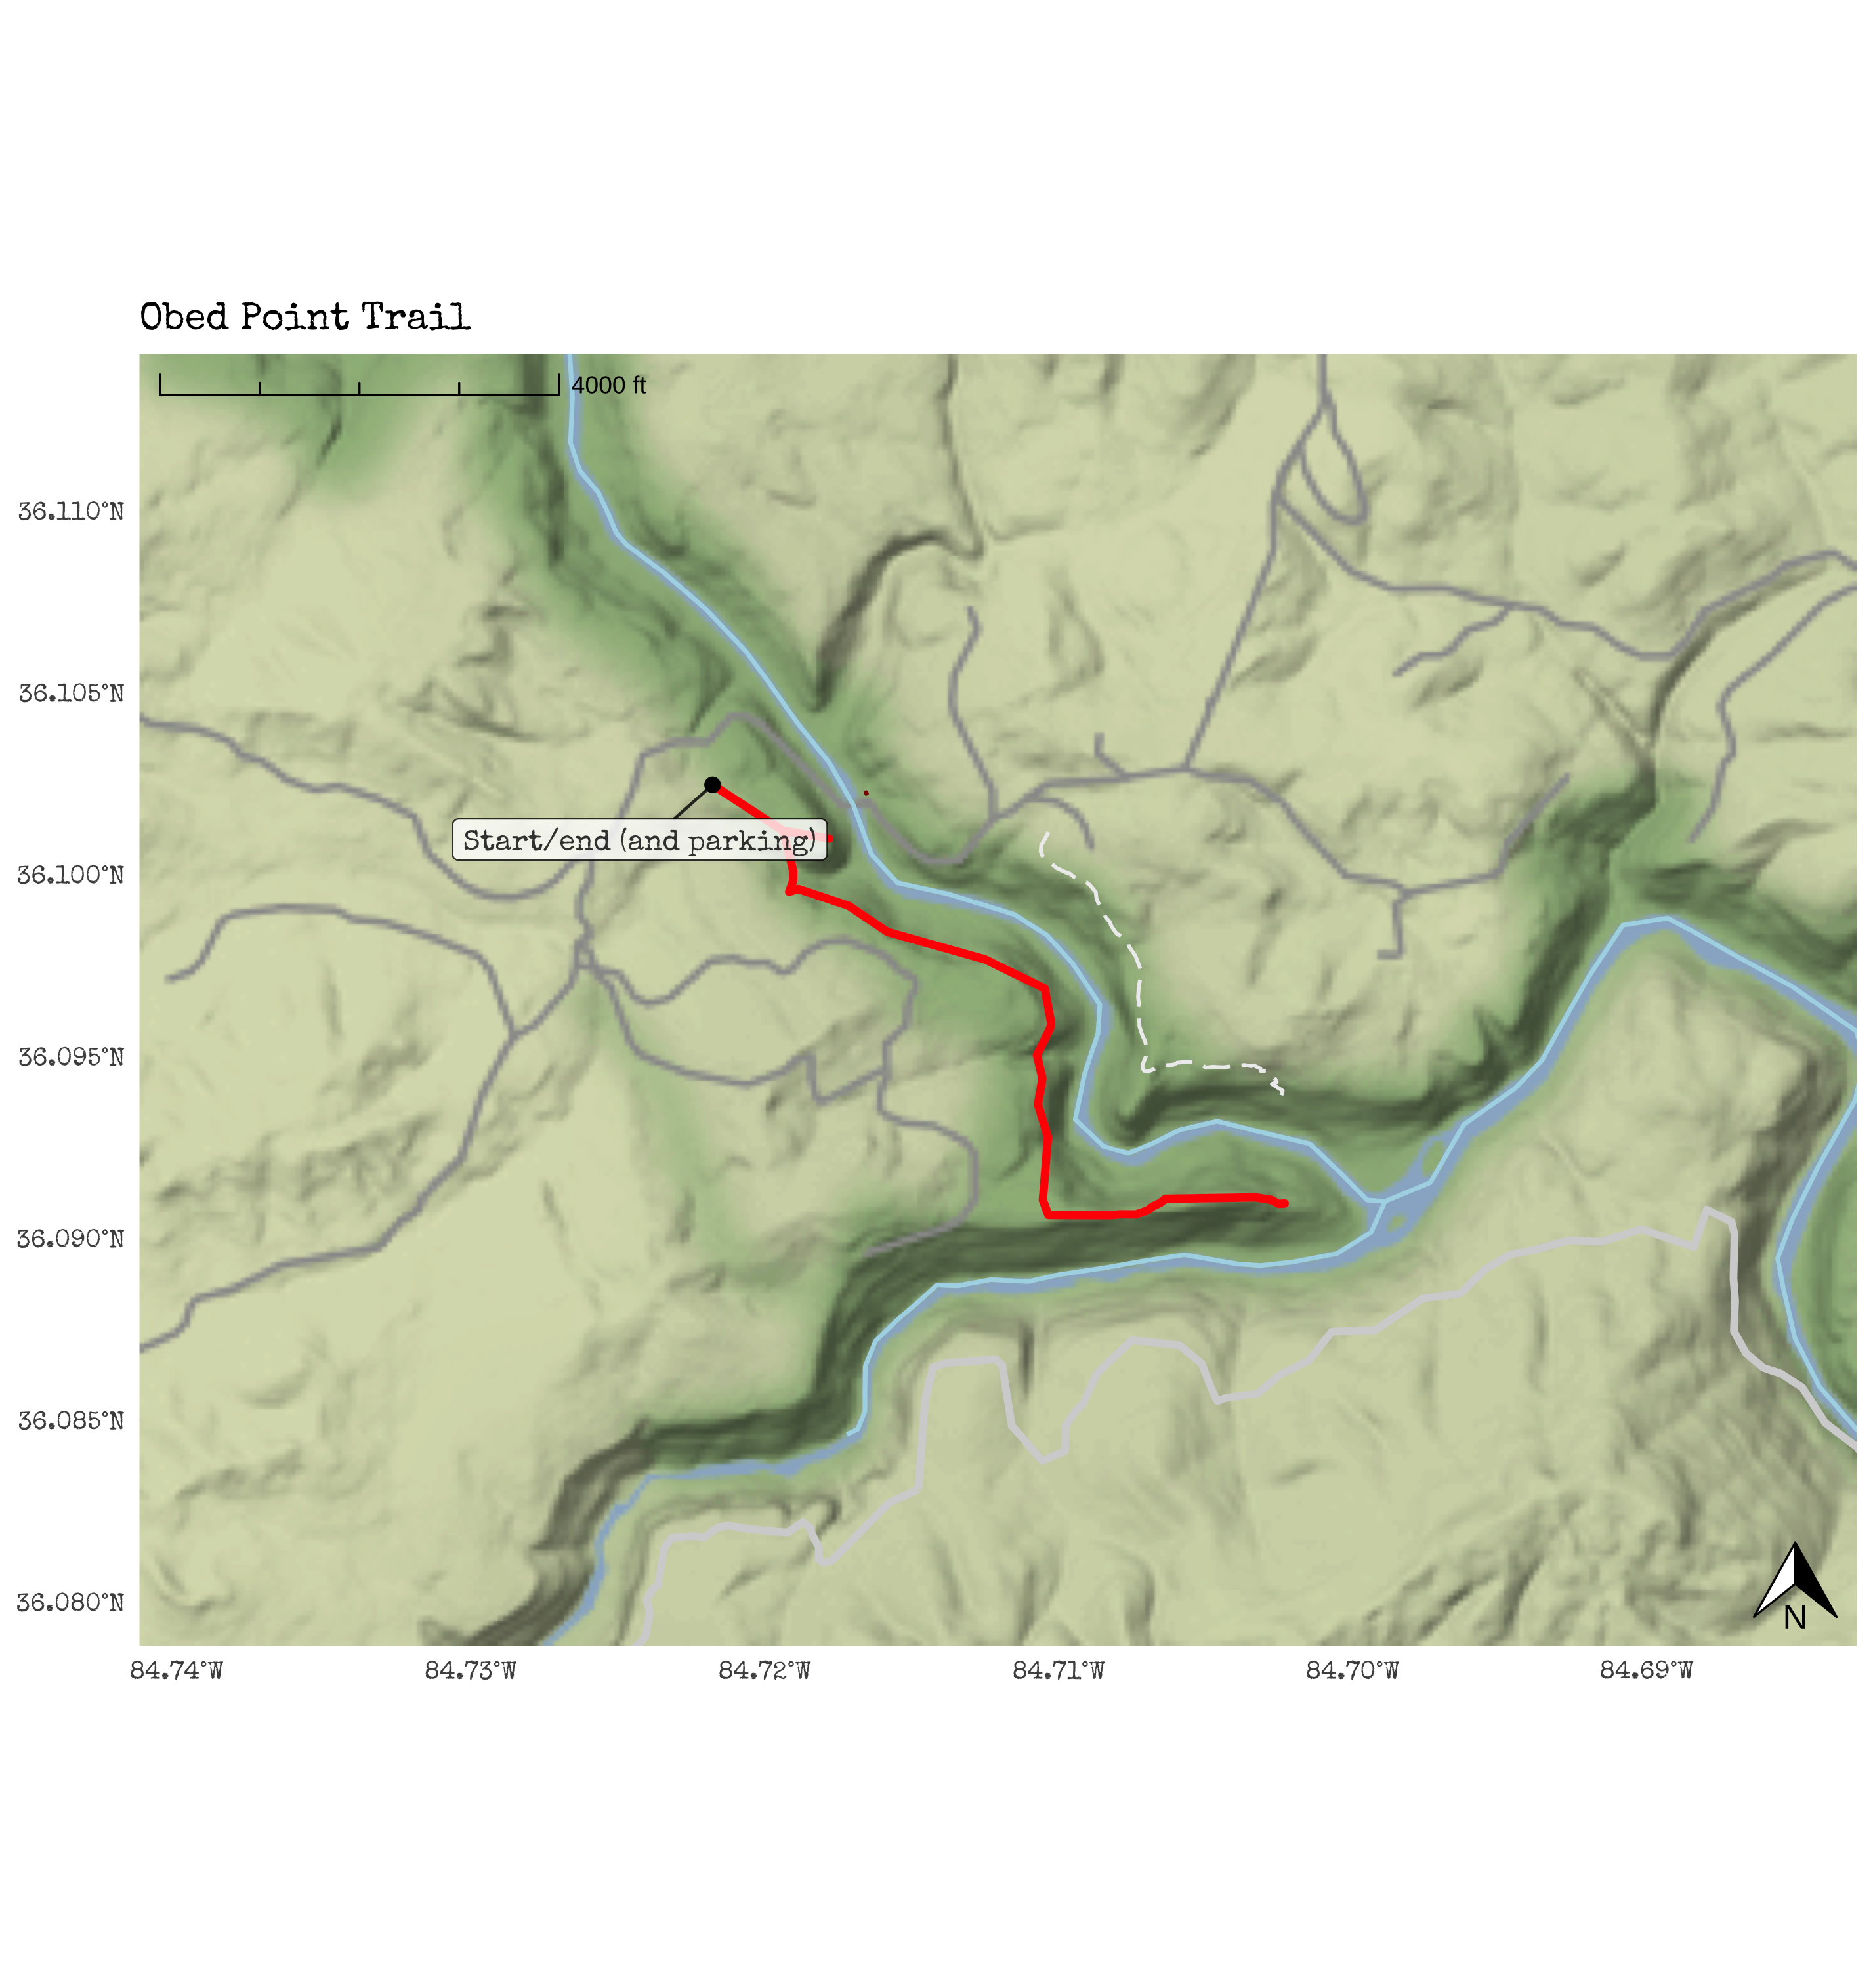
\includegraphics[width=39.64in]{/Users/joshuarosenberg/little-kids-big-adventures/output/obed-point-trail-map} \caption{Seven Islands Loop Trail Map}\label{fig:unnamed-chunk-23}
\end{figure}

\hypertarget{trail-description-7}{%
\section{Trail Description}\label{trail-description-7}}

\hypertarget{nearby-7}{%
\section{Nearby}\label{nearby-7}}

\hypertarget{emory-falls-frozen-head}{%
\chapter{Emory Falls (Frozen Head)}\label{emory-falls-frozen-head}}

\hypertarget{trail-information-8}{%
\section{Trail Information}\label{trail-information-8}}

\hypertarget{ratings-3}{%
\subsection{Ratings}\label{ratings-3}}

\begin{tabular}{l|r|r|r|r}
\hline
Hike Name & Beauty & Accessibility & Amenities & Challenge\\
\hline
Emory Falls & 4 & 3 & 4 & 2\\
\hline
\end{tabular}

\hypertarget{basic-characteristics-8}{%
\subsection{Basic Characteristics}\label{basic-characteristics-8}}

Location: Frozen Head State Park\\
Region: The Cumberland Plateau\\
Distance: 2.43 (mi.)\\
Elevation (Ascend): 480 (ft.)\\
Max. Elevation: 2036 (ft.)

\hypertarget{overview-8}{%
\section{Overview}\label{overview-8}}

\hypertarget{map-8}{%
\section{Map}\label{map-8}}

\begin{figure}
\includegraphics[width=39.64in]{/Users/joshuarosenberg/little-kids-big-adventures/output/emory-falls-map} \caption{Seven Islands Loop Trail Map}\label{fig:unnamed-chunk-25}
\end{figure}

\hypertarget{trail-description-8}{%
\section{Trail Description}\label{trail-description-8}}

\hypertarget{nearby-8}{%
\section{Nearby}\label{nearby-8}}

\hypertarget{twin-arches}{%
\chapter{Twin Arches}\label{twin-arches}}

\hypertarget{trail-information-9}{%
\section{Trail Information}\label{trail-information-9}}

\hypertarget{ratings-4}{%
\subsection{Ratings}\label{ratings-4}}

\begin{tabular}{l|r|r|r|r}
\hline
Hike Name & Beauty & Accessibility & Amenities & Challenge\\
\hline
Twin Arches Loop & 5 & 2 & 2 & 3\\
\hline
\end{tabular}

\hypertarget{basic-characteristics-9}{%
\subsection{Basic Characteristics}\label{basic-characteristics-9}}

Location: Twin Arches State Recreation Area\\
Region: The Cumberland Plateau\\
Distance: 1.15 (mi.)\\
Elevation (Ascend): 297 (ft.)\\
Max. Elevation: 1574 (ft.)

\hypertarget{overview-9}{%
\section{Overview}\label{overview-9}}

\hypertarget{map-9}{%
\section{Map}\label{map-9}}

\begin{figure}
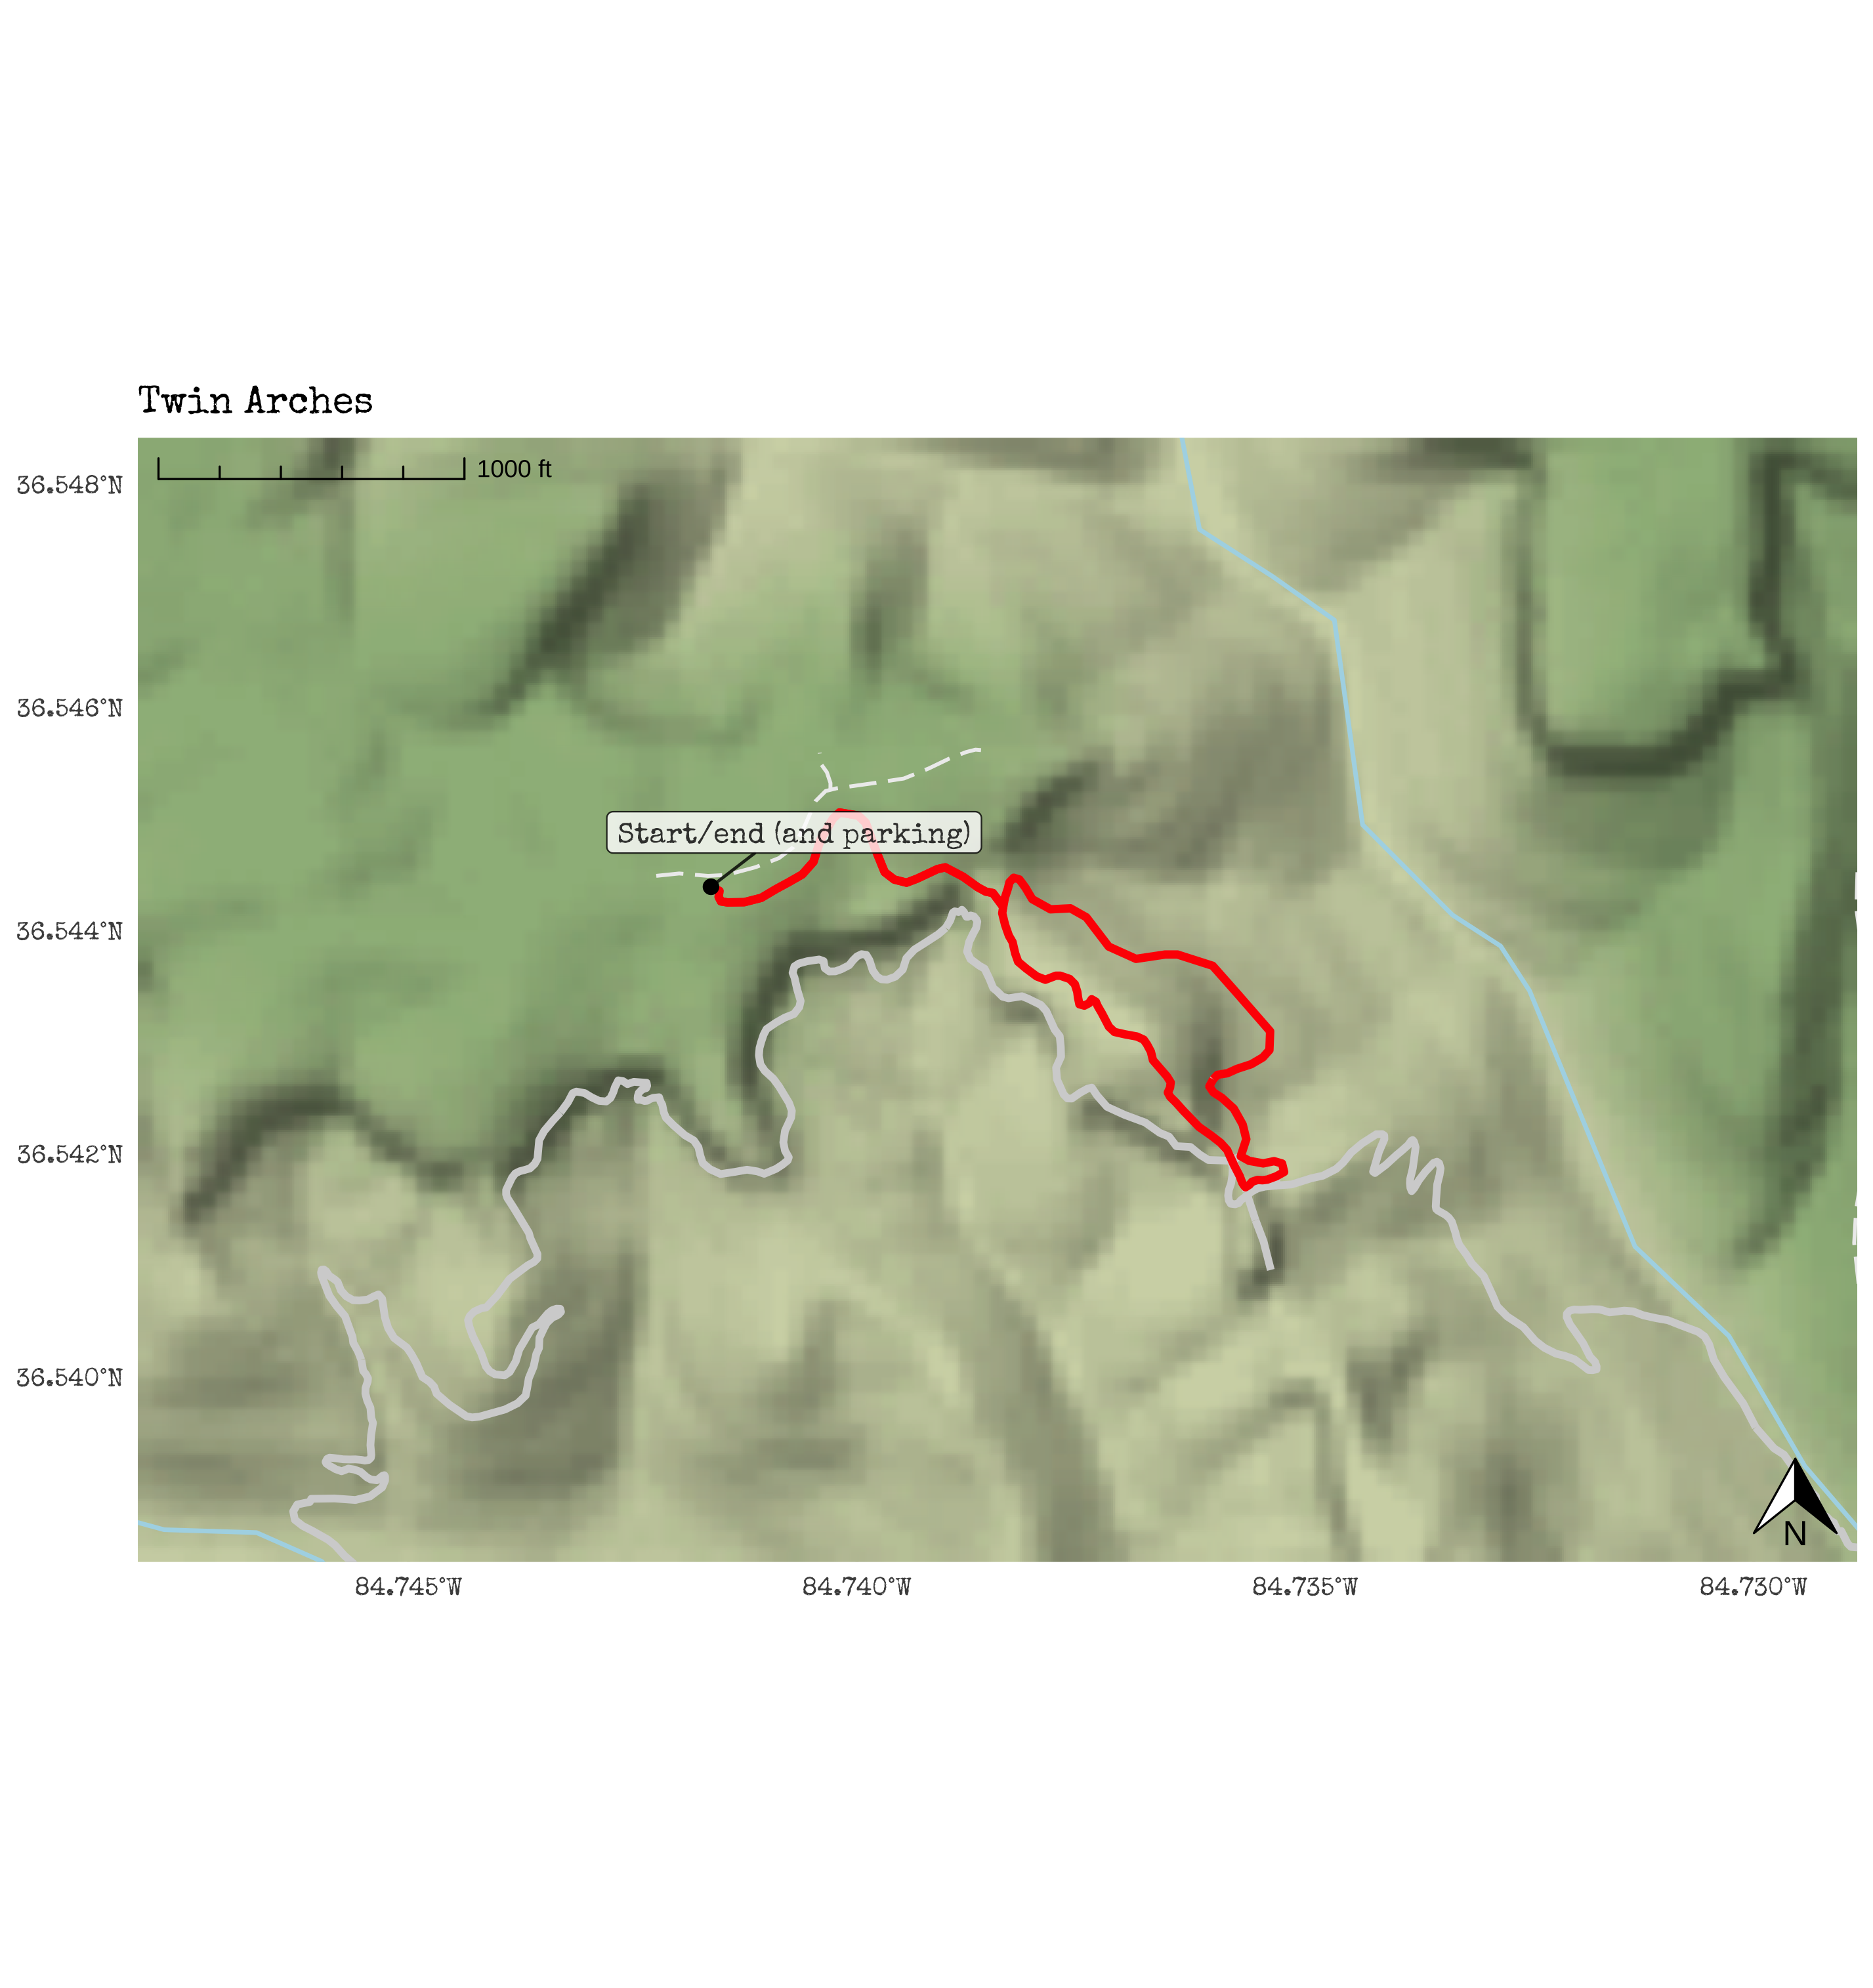
\includegraphics[width=39.64in]{/Users/joshuarosenberg/little-kids-big-adventures/output/twin-arches-loop-map} \caption{Seven Islands Loop Trail Map}\label{fig:unnamed-chunk-27}
\end{figure}

\hypertarget{trail-description-9}{%
\section{Trail Description}\label{trail-description-9}}

\hypertarget{nearby-9}{%
\section{Nearby}\label{nearby-9}}

\hypertarget{honey-creek-big-south-fork}{%
\chapter{Honey Creek (Big South Fork)}\label{honey-creek-big-south-fork}}

\hypertarget{trail-information-10}{%
\section{Trail Information}\label{trail-information-10}}

\hypertarget{ratings-5}{%
\subsection{Ratings}\label{ratings-5}}

\begin{tabular}{l|r|r|r|r}
\hline
Hike Name & Beauty & Accessibility & Amenities & Challenge\\
\hline
Honey Creek & 5 & 2 & 1 & 5\\
\hline
\end{tabular}

\hypertarget{basic-characteristics-10}{%
\subsection{Basic Characteristics}\label{basic-characteristics-10}}

Location: Big South Fork National River and Recreation Area\\
Region: The Cumberland Plateau\\
Distance: 4.4 (mi.)\\
Elevation (Ascend): 962 (ft.)\\
Max. Elevation: 1587 (ft.)

\hypertarget{overview-10}{%
\section{Overview}\label{overview-10}}

\hypertarget{map-10}{%
\section{Map}\label{map-10}}

\begin{figure}
\includegraphics[width=39.64in]{/Users/joshuarosenberg/little-kids-big-adventures/output/honey-creek-loop-map} \caption{Seven Islands Loop Trail Map}\label{fig:unnamed-chunk-29}
\end{figure}

\hypertarget{trail-description-10}{%
\section{Trail Description}\label{trail-description-10}}

\hypertarget{nearby-10}{%
\section{Nearby}\label{nearby-10}}

\hypertarget{bandy-creek-big-south-fork}{%
\chapter{Bandy Creek (Big South Fork)}\label{bandy-creek-big-south-fork}}

\hypertarget{trail-information-11}{%
\section{Trail Information}\label{trail-information-11}}

\hypertarget{ratings-6}{%
\subsection{Ratings}\label{ratings-6}}

\begin{tabular}{l|r|r|r|r}
\hline
Hike Name & Beauty & Accessibility & Amenities & Challenge\\
\hline
Bandy Creek & 4 & 2 & 4 & 3\\
\hline
\end{tabular}

\hypertarget{basic-characteristics-11}{%
\subsection{Basic Characteristics}\label{basic-characteristics-11}}

Location: Big South Fork National River and Recreation Area\\
Region: The Cumberland Plateau\\
Distance: 3.67 (mi.)\\
Elevation (Ascend): 363 (ft.)\\
Max. Elevation: 1601 (ft.)

\hypertarget{overview-11}{%
\section{Overview}\label{overview-11}}

\hypertarget{map-11}{%
\section{Map}\label{map-11}}

\begin{figure}
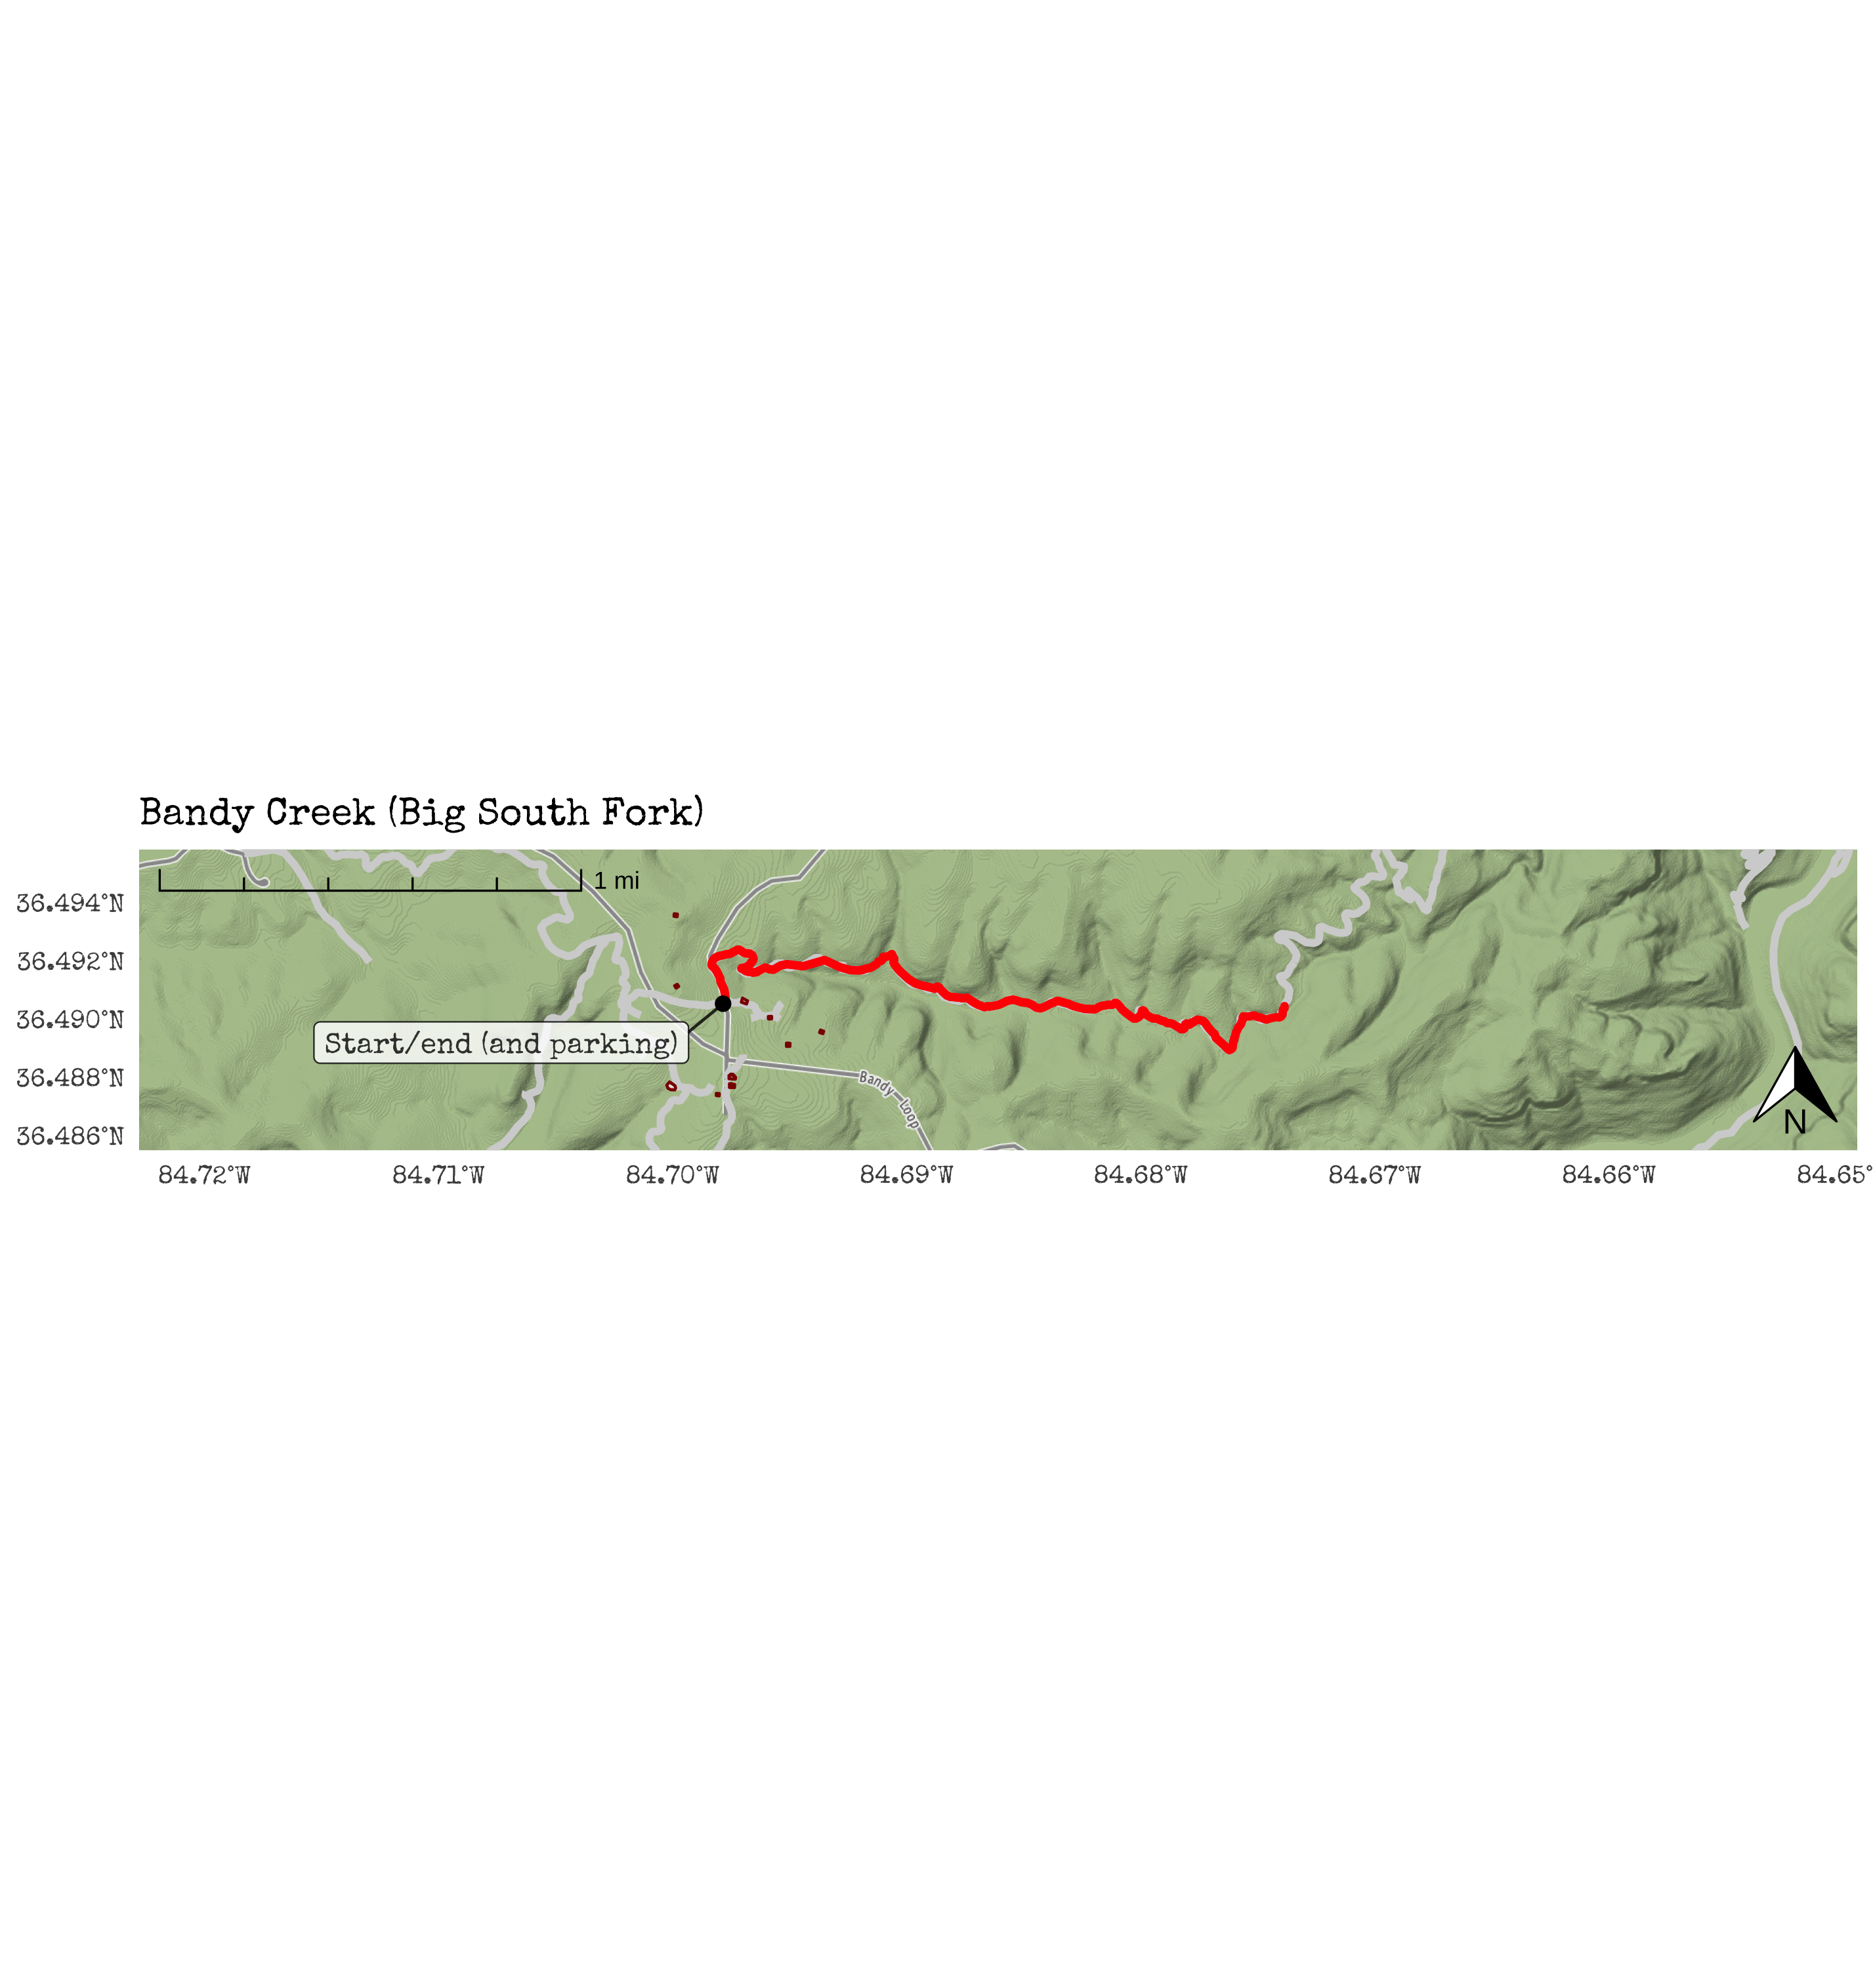
\includegraphics[width=39.64in]{/Users/joshuarosenberg/little-kids-big-adventures/output/bandy-creek-fall-branch-falls-map} \caption{Seven Islands Loop Trail Map}\label{fig:unnamed-chunk-31}
\end{figure}

\hypertarget{trail-description-11}{%
\section{Trail Description}\label{trail-description-11}}

\hypertarget{nearby-11}{%
\section{Nearby}\label{nearby-11}}

\hypertarget{part-the-smokies}{%
\part{The Smokies}\label{part-the-smokies}}

\hypertarget{little-river-loop}{%
\chapter{Little River Loop}\label{little-river-loop}}

\hypertarget{trail-information-12}{%
\section{Trail Information}\label{trail-information-12}}

\hypertarget{ratings-7}{%
\subsection{Ratings}\label{ratings-7}}

\begin{tabular}{l|r|r|r|r}
\hline
Hike Name & Beauty & Accessibility & Amenities & Challenge\\
\hline
Little River Loop & 4 & 3 & 3 & 3\\
\hline
\end{tabular}

\hypertarget{basic-characteristics-12}{%
\subsection{Basic Characteristics}\label{basic-characteristics-12}}

Location: Great Smoky Mountains National Park\\
Region: The Smokies and Beyond\\
Distance: 5.49 (mi.)\\
Elevation (Ascend): 996 (ft.)\\
Max. Elevation: 3042 (ft.)

\hypertarget{overview-12}{%
\section{Overview}\label{overview-12}}

\hypertarget{map-12}{%
\section{Map}\label{map-12}}

\begin{figure}
\includegraphics[width=39.64in]{/Users/joshuarosenberg/little-kids-big-adventures/output/little-river-loop-map} \caption{Seven Islands Loop Trail Map}\label{fig:unnamed-chunk-33}
\end{figure}

\hypertarget{trail-description-12}{%
\section{Trail Description}\label{trail-description-12}}

\hypertarget{nearby-12}{%
\section{Nearby}\label{nearby-12}}

\hypertarget{abrams-creek}{%
\chapter{Abrams Creek}\label{abrams-creek}}

\hypertarget{basic-information}{%
\section{Basic Information}\label{basic-information}}

\hypertarget{characteristics}{%
\subsection{Characteristics}\label{characteristics}}

Location: Great Smoky Mountains National Park\\
Region: The Smokies and Beyond\\
Distance: 5.78 mi.\\
Ascent: 991 ft.\\
Max. Elevation: 1425 ft.

\hypertarget{highlights}{%
\subsection{Highlights}\label{highlights}}

\begin{itemize}
\tightlist
\item
  Accessible, beautiful location in the national park
\item
  Mostly flat walking along a large waterway (practically a river), Abrams Creek
\item
  Many opportunities to splash around in Abrams Creek or the smaller creeks that criss-cross the trail
\end{itemize}

\hypertarget{ratings-8}{%
\subsection{Ratings}\label{ratings-8}}

\begin{table}
\centering
\begin{tabular}[t]{l|r|r|r|r}
\hline
Hike Name & Beauty & Accessibility & Amenities & Challenge\\
\hline
Abrams Creek & 4 & 2 & 3 & 2\\
\hline
\end{tabular}
\end{table}

\hypertarget{trail-map}{%
\subsection{Trail Map}\label{trail-map}}

\begin{figure}
\includegraphics[width=39.64in]{/Users/joshuarosenberg/little-kids-big-adventures/output/abrams-creek-map} \caption{Abrams Creek Trail Map}\label{fig:unnamed-chunk-36}
\end{figure}

\hypertarget{trail-overview}{%
\section{Trail Overview}\label{trail-overview}}

Abrams Creek is a great place to start exploring if you live in or around Knoxville.
Though accessible, it's also beautiful. This was the first place we traveled as
a family in the Smokies. The single best thing we can say about Abrams Creek is
that we always seem to have fun when we go there.

This trail is listed as a quite long---5.78 miles.
But, there are many ways to shorten the hike, and we often head to the Creek or
Backcountry Site (listed on the map), at 1.0 and 1.3 miles from the start of
the hike, respectively. Both include plenty of highlights. The full hike ends
at \emph{another} backcountry site; it's one of the best in the entire national
park to camp overnight, and it also makes a great place to rest, snack or
picnic, and hang out.

\begin{rmdhistory}
You might be thinking - as we were - that the `Abrams' in the name
Abrams Creek was a reference to Abraham (of the Old Testament). Many
sources note that Abrams Creek is named for a Cherokee Chief who was
colloquially known by the individuals of European ancestry as `Old
Abram'. He was a chief for an area around Chilhowee, an important
Cherokee village, around the end of the 18th century. See @fink1934smoky
(cited in @dunn1976cades) for more information.
\end{rmdhistory}

\hypertarget{getting-there}{%
\section{Getting There}\label{getting-there}}

The drive there is also \emph{mostly} easy. Getting to Abrams Creek involves driving
south from Knoxville past the Tyson-McGee Airport and then Maryville.
Soon after leaving the outskirts of Maryville, the road climbs up Chilhowee
Mountain, atop which is the beautiful Foothills Parkway; the road becomes quite
steep, but it is---of course---paved and is still accessible. After crossing
under the Foothills Parkway, you drive down into the area outside of the Abrams
Creek Trailhead and Campground.

The most reliable way to find the trailhead via Google Maps or other mapping
tools is to search for `Abrams Creek Campground' in Tallassee, TN.

It never seems to become crowded at Abrams Creek, but parking can be \emph{a bit}
confusing. This is because the campground is further along the same road the
trailhead is on. Also, there are two areas to park for the trailhead:

\begin{itemize}
\tightlist
\item
  One place to park is near the large sign with maps of this area of the national park\\
\item
  The other is right by the gate to the campground
\end{itemize}

We usually park by the gate.

\hypertarget{trail-description-13}{%
\section{Trail Description}\label{trail-description-13}}

This trail is an out-and-back, starting at the trailhead parking area and heading out as far
along the trail as you wish---then returning back to the beginning.

Starting from the parking area, walk along the road beside Abrams Creek. The
campground is so small (and almost never full), and it is very rare that you
will encounter a car on the walk along the road.

\begin{figure}

{\centering 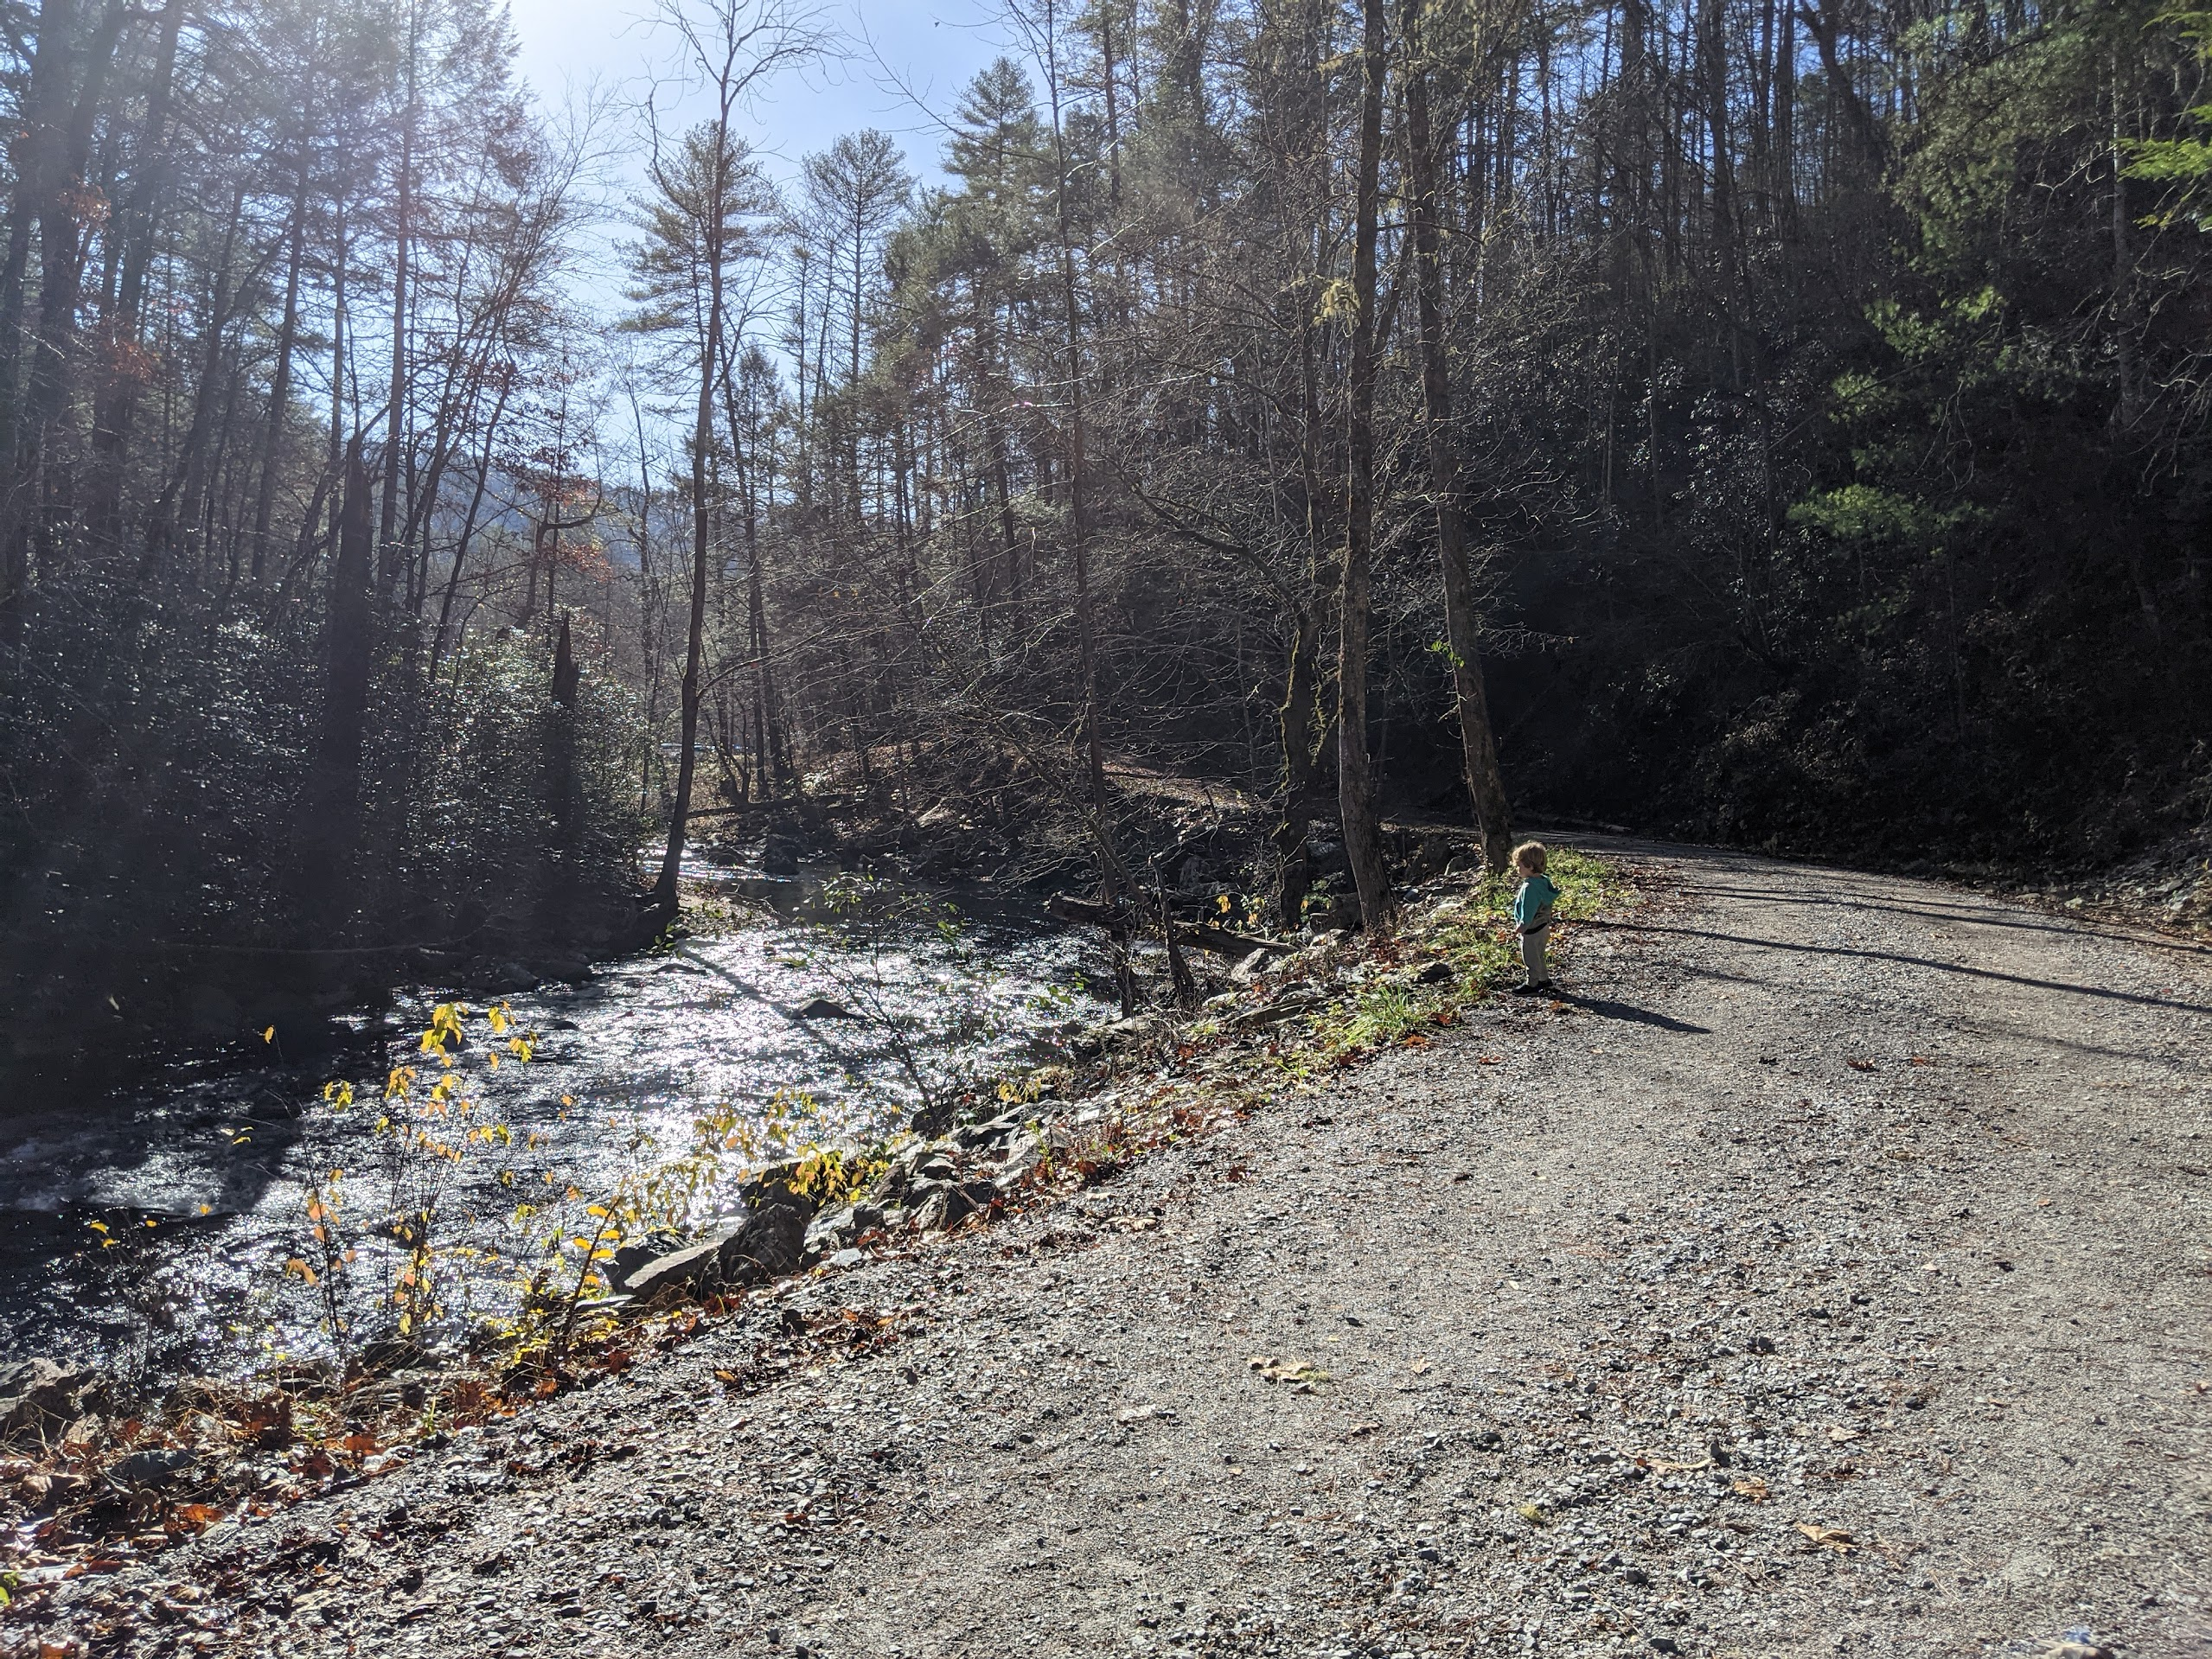
\includegraphics[width=0.9\linewidth]{/Users/joshuarosenberg/little-kids-big-adventures/img/abrams-road} 

}

\caption{The road to Abrams Creek}\label{fig:unnamed-chunk-38}
\end{figure}

The littlest adventure involves walking from the trailhead to the \emph{Campground}
(see the marker on the map). This may not sound like much, but it's actually a great walk
along the creek on a wide, gravel road. Moreover, the campground as the
campground- like Abrams Creek - is almost never busy, and it's a great spot to
rest by picnic tables and hang out around the creek. The campground is around
\textbf{.40 miles} from the parking area, making a trip there and back a little less
than a mile.

\begin{rmdscience}
Do you see the tall pine trees here at the campground? Many of them are
\textbf{Eastern Hemlocks}, one of the tallest trees in the Eastern
United States. Hemlocks can be identified by their \emph{flat} needles
that exhibit a \emph{flat} arrangement on the trees' branches. They can
take 250 to 300 years to reach maturity and can live for an astonishing
800 years or more. They can grow to far taller than 150 feet. The
tallest Eastern Hemlock in the world is in the Smokies and
\href{https://www.monumentaltrees.com/en/trees/tsugacanadensis/records/}{is
around 170 feet tall}!

You may notice that some of the trees have what appears to be a painted
marking on their base. The National Park Service (who manage the
national park) has undertaken an effort to treat Eastern Hemlock trees
to prevent them from being infected by the \emph{Hemlock Wooly Adelgid},
an insect that is considered to be an invasive species--and one that
harms many (untreated) Hemlock trees.

Fortunately, the treatment is relatively easy to administer to trees; a
chemical very similar to that in anti-tick sprays for pets (like dogs)
is dissolved in water, the needles and soil around the base of the trees
(which is known as ``duff'') are lightly moved, and around a gallon or
more of the solution is poured along the base. This treatment is
effective at preventing the trees from being infected for five or more
years. The park service has treated more than 200,000 trees in this way.
Learn more about the Hemlock Wooly Adelgid and its prevention in
@nps\_hwa.

Learn more about Eastern Hemlocks in @godman2021hemlock.
\end{rmdscience}

\begin{figure}

{\centering 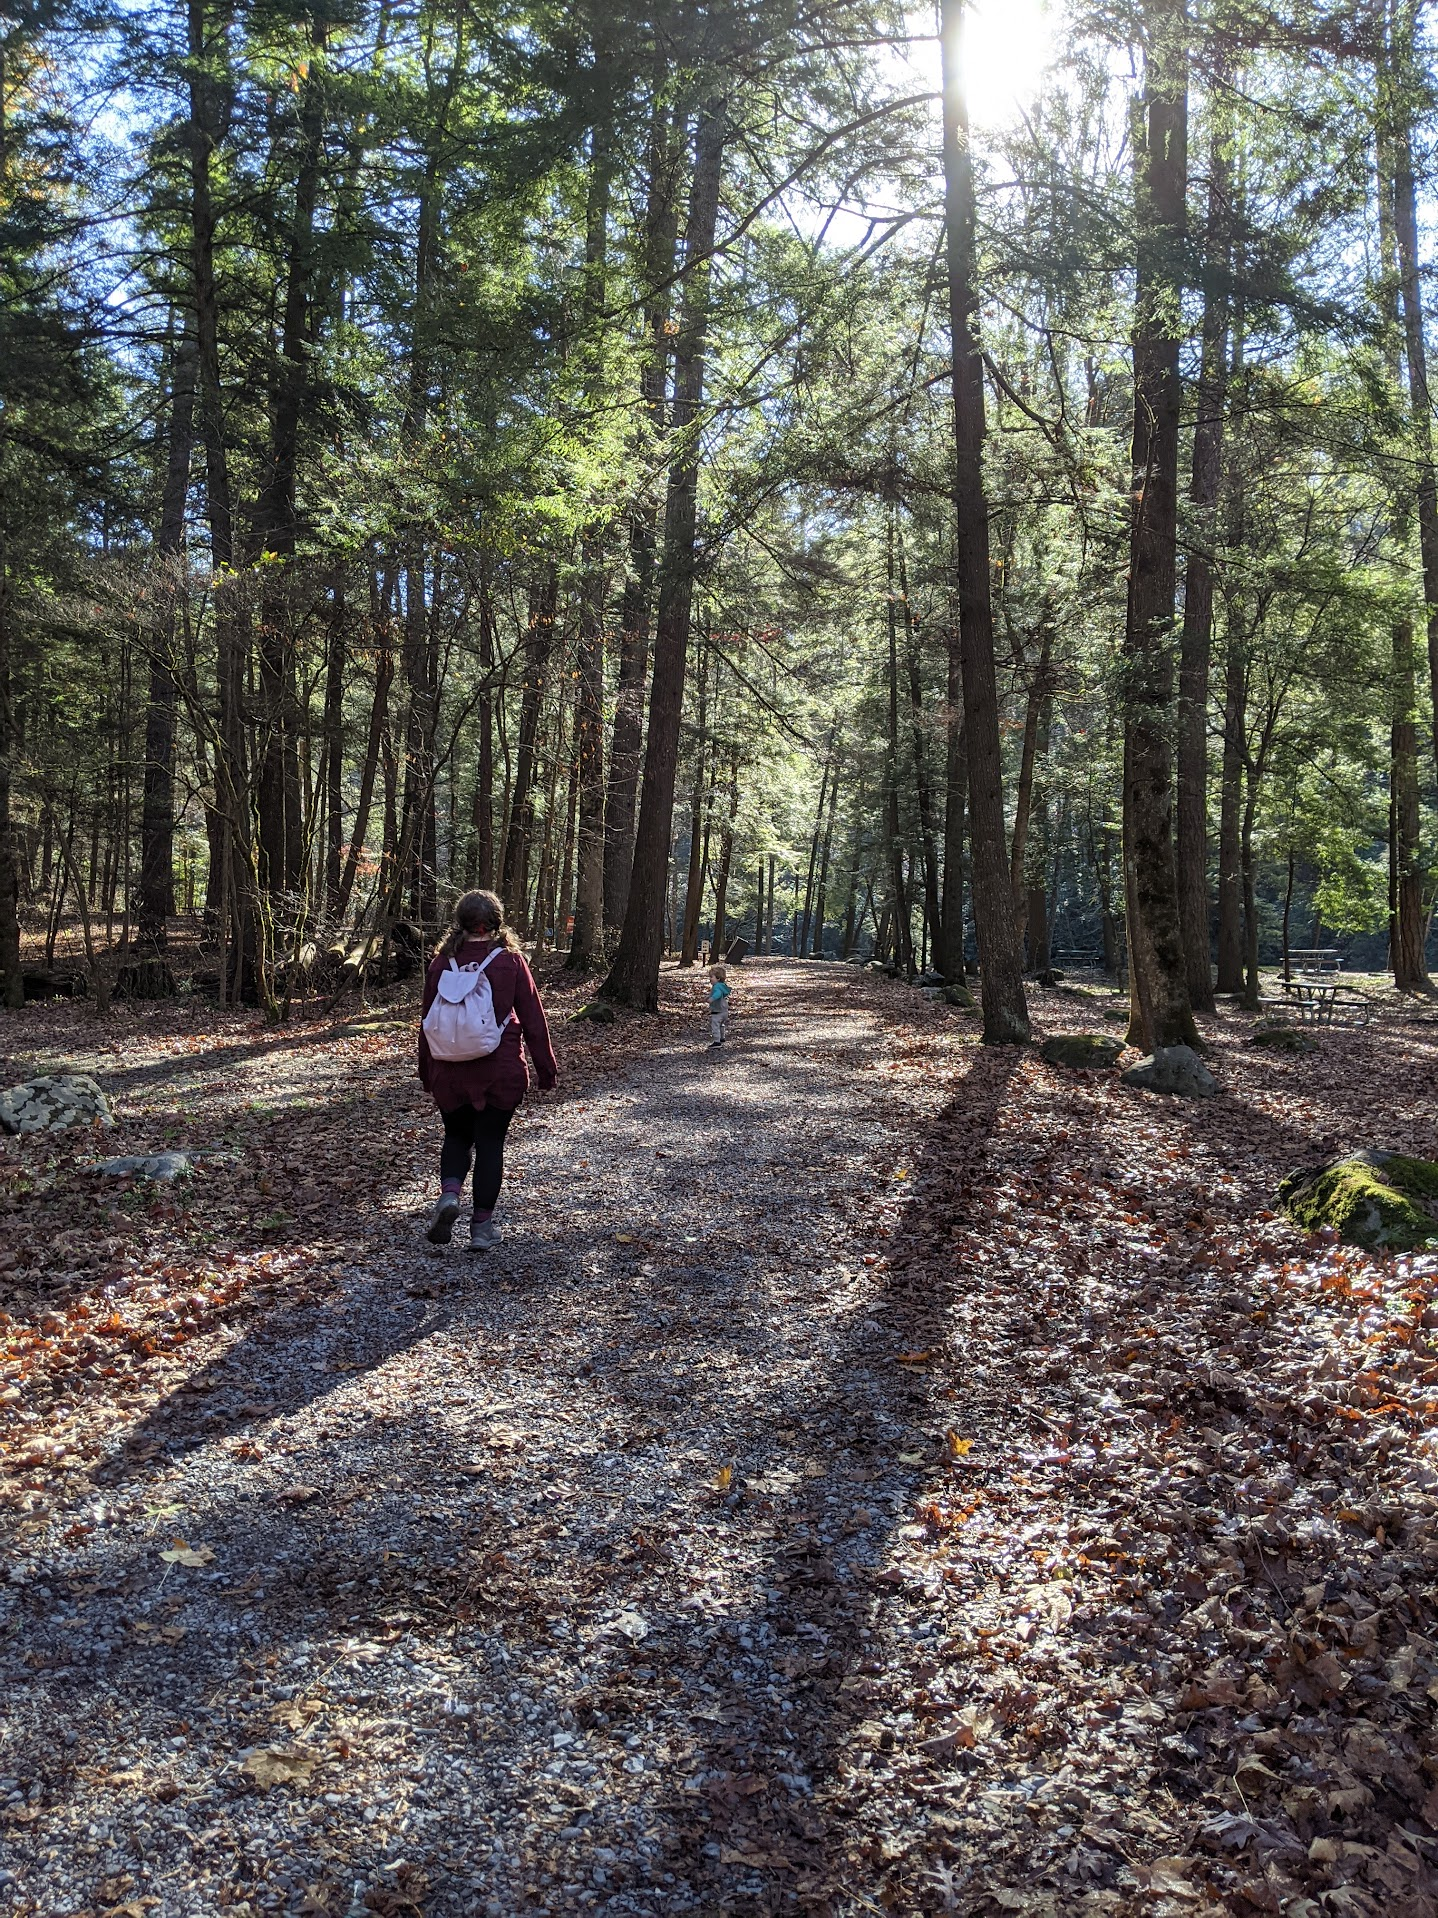
\includegraphics[width=0.9\linewidth]{/Users/joshuarosenberg/little-kids-big-adventures/img/abrams-campground-walking} 

}

\caption{The campground at Abrams Creek}\label{fig:unnamed-chunk-40}
\end{figure}

Walking on from the campground, you will enter a densely wooded area covered
by the branches and needles of tall pine trees. Soon, you'll gently ascend an
incline, but the climbing is never protracted.

\begin{figure}

{\centering \includegraphics[width=0.9\linewidth]{/Users/joshuarosenberg/little-kids-big-adventures/img/abrams-hike-clear} 

}

\caption{The Cane Creek Trail exiting the campground}\label{fig:unnamed-chunk-41}
\end{figure}

After climbing, you'll descend to the first crossing with Kingfisher Creek at \textbf{1.0 mile} (labeled as ``Creek'' on the map).

\begin{figure}

{\centering 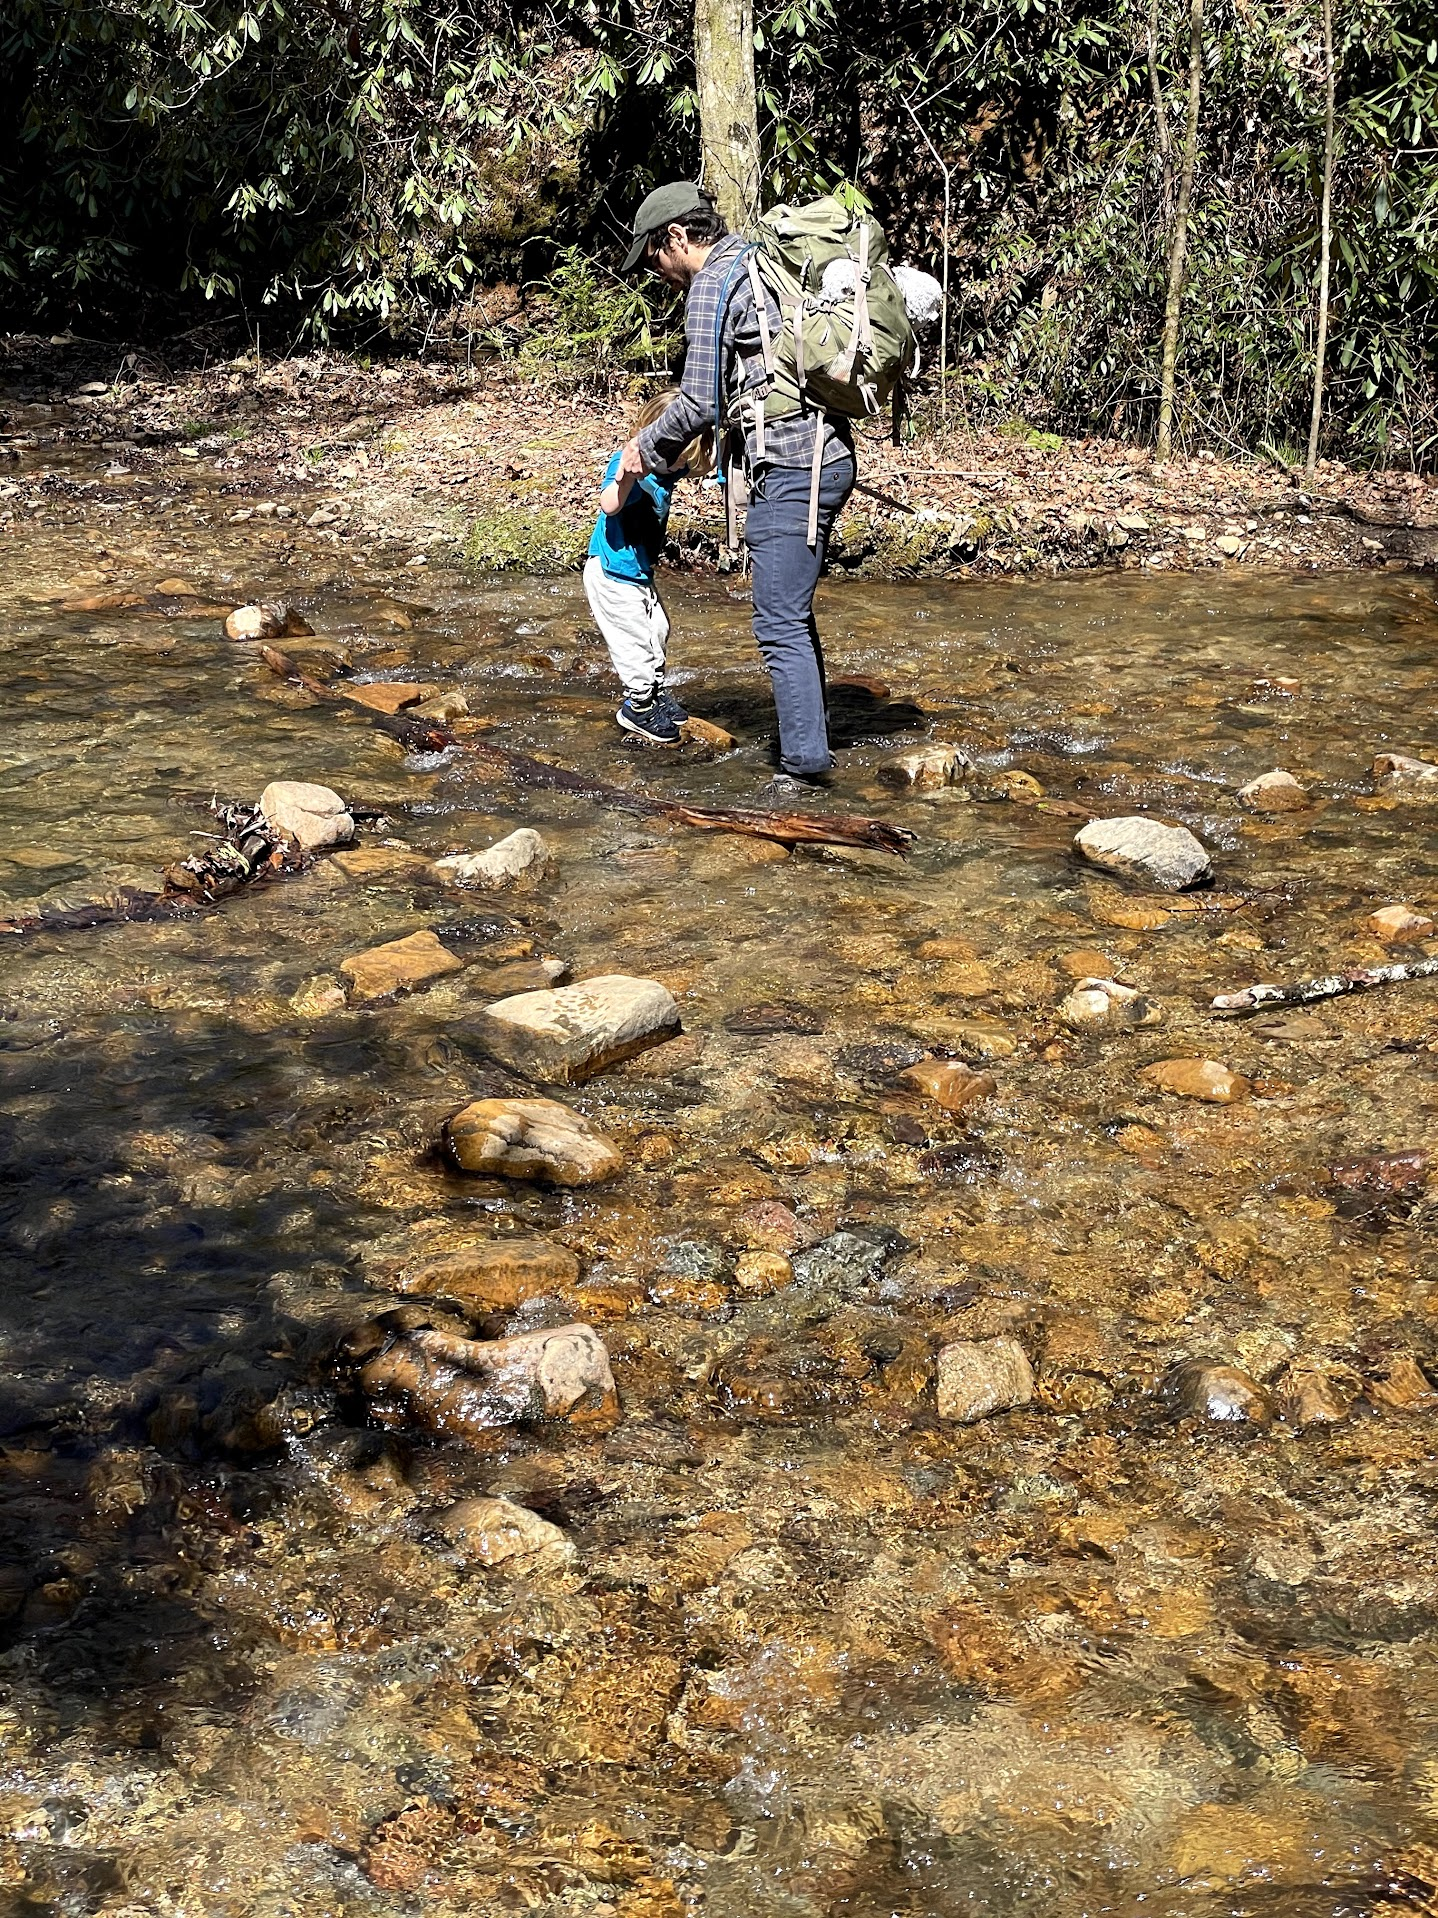
\includegraphics[width=0.9\linewidth]{/Users/joshuarosenberg/little-kids-big-adventures/img/abrams-high-water-crossing} 

}

\caption{Crossing Kingfisher Creek}\label{fig:unnamed-chunk-42}
\end{figure}

This is a fun place to rest and snack. To continue on, you'll need to cross the
creek; sometimes, higher water here means we stop here and turn around. At its
highest, the water is about six inches deep - nothing dangerous, but it can be
difficult to safely and easily walk across the rocks or branches there that
ease the crossing.

\begin{rmdtip}
One way to make creek crossings easier is to grab a large stick to help
you to maintain balance as you walk across rocks or logs. Trekking polls
(available at outdoors stores) are also great for this purpose, but a
stick will do just fine.
\end{rmdtip}

After crossing Kingfisher Creek for the first time, another crossing (of this
same creek) awaits around 100 yards further from the first crossing. This one
is sometimes a little bit easier than the first crossing.

The trail continues to \emph{Backcountry Site \#1} at \textbf{1.3 miles} from the trail
head. The `\#1' refers to this site's number among all of the backcountry sites
in the park: there are around 70, total (the number changes as sites are added,
removed, or moved to ensure that the areas around the sites are not impacted
too negatively by their frequent use), and this one happens to be numbered as
the first! This is a fairly frequently-used backcountry campsite, one used by
those backpacking and camping overnight; the national park only allows camping
at designated backcountry sites (such as this one) or sites at frontcountry
campgrounds--like the one you passed earlier.

This is another great place to stop and rest. If you so choose, you can
continue from here. Note the trail sign that is immediately before the
backcountry site; it marks the intersection between the \emph{Cooper Road Trail},
which you have been on, and the \emph{Little Bottoms Trail}, which branches from the
Cooper Road Trail here. To continue further, take the Little Bottoms Trail.
You'll soon cross a (small) creek and begin to climb---the steepest climb of
this entire trail and a quite steep (albeit brief) climb by any metric. At the
top of the climb atop this ridge, you'll find another good spot to stop to rest
at \textbf{1.5 miles}.

\begin{figure}

{\centering 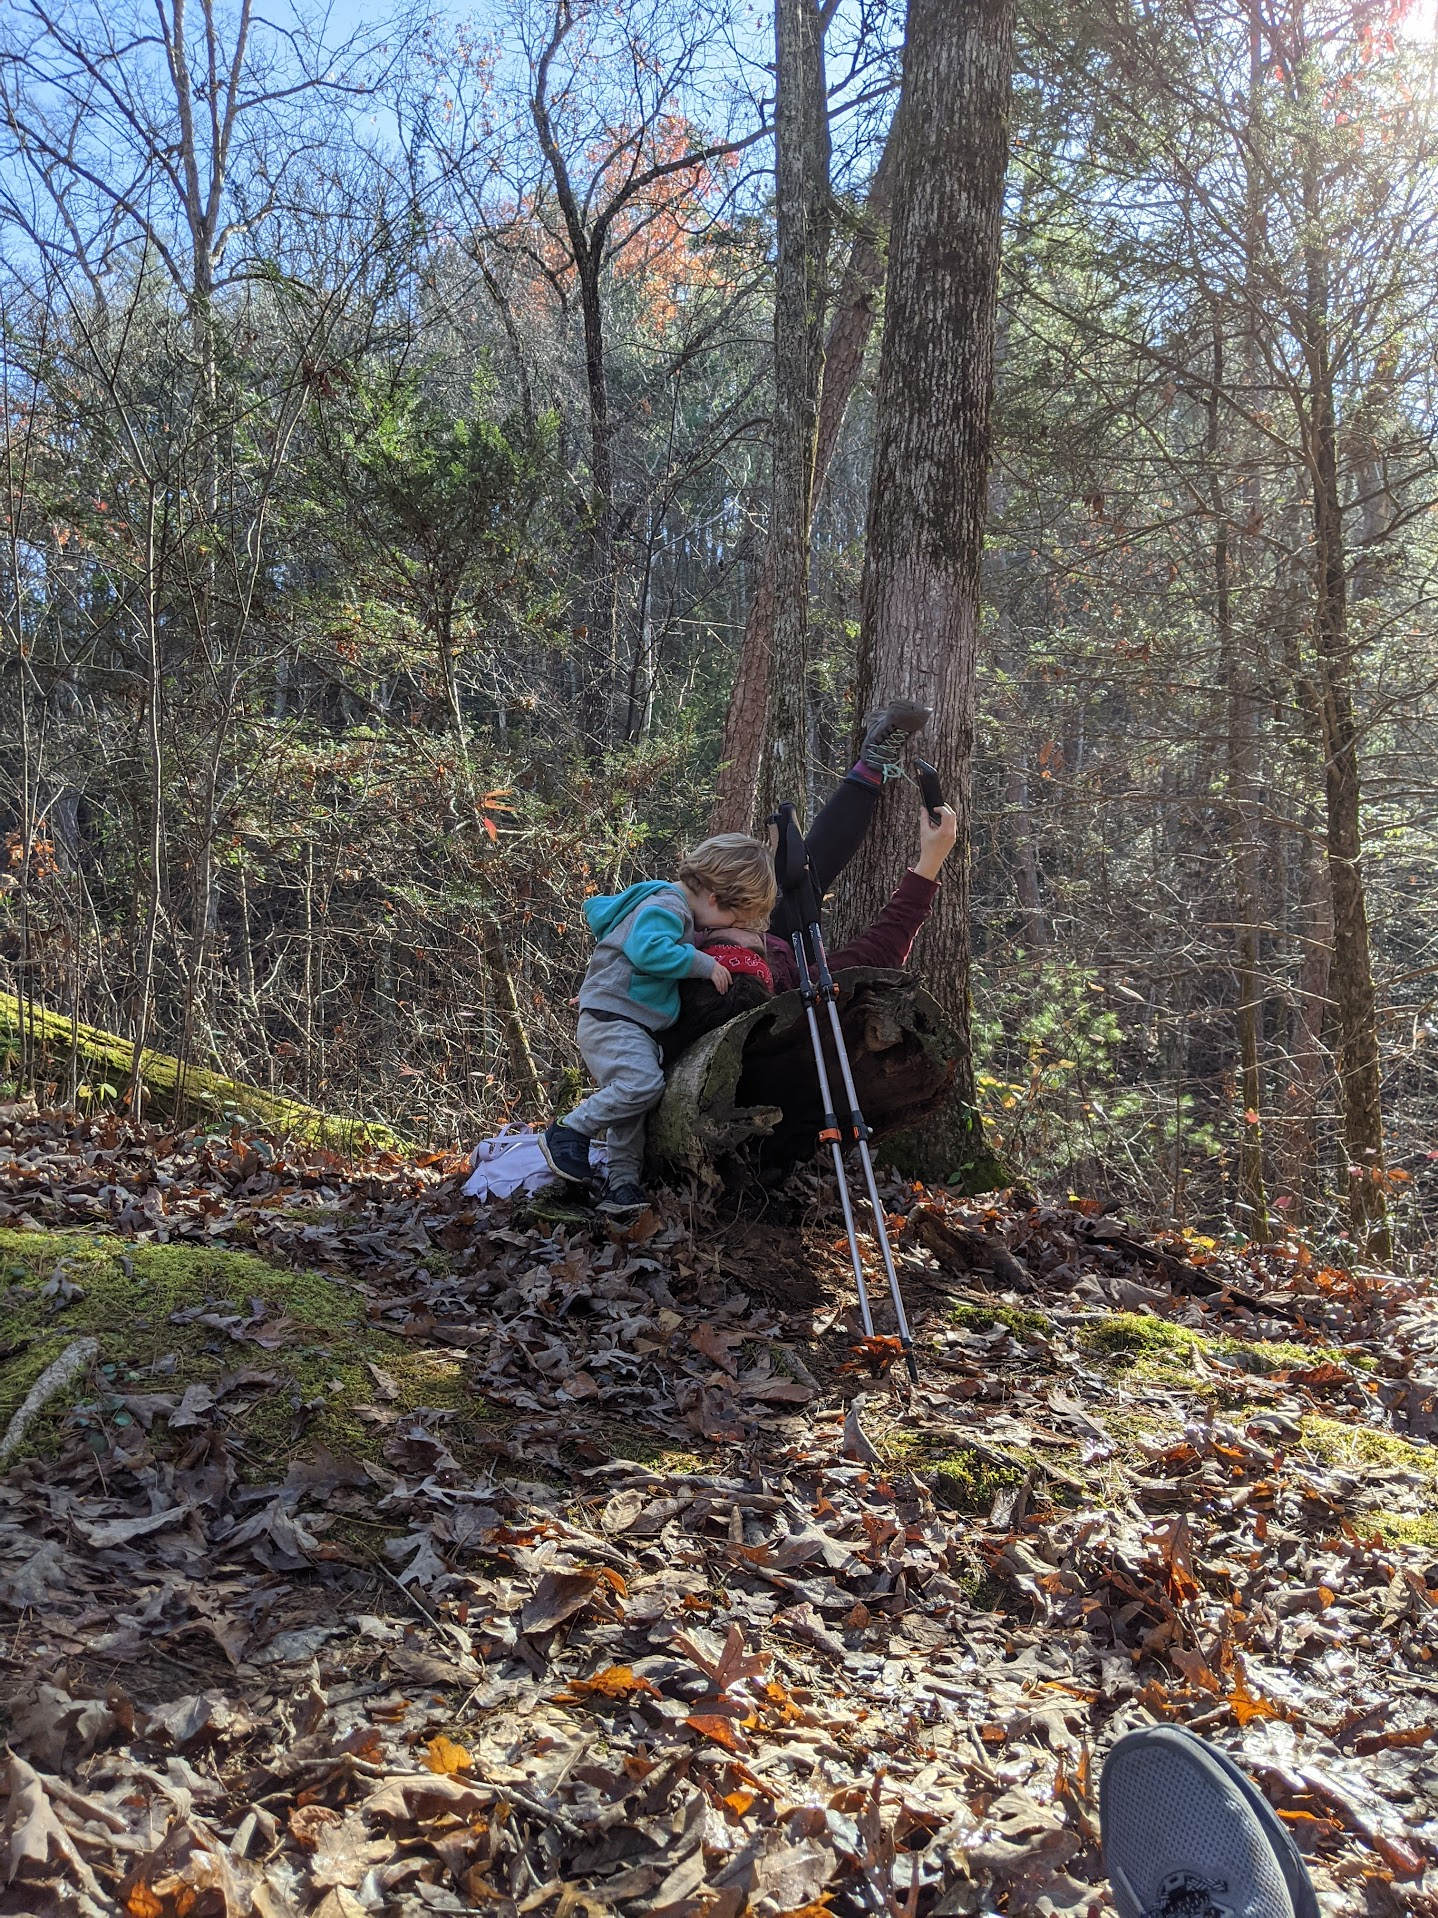
\includegraphics[width=0.9\linewidth]{/Users/joshuarosenberg/little-kids-big-adventures/img/abrams-log} 

}

\caption{Spot to rest on top of the ridge}\label{fig:unnamed-chunk-44}
\end{figure}

Continue onward along the ridge that you just climbed, soon reaching an
overlook at \textbf{1.6 miles}.

\begin{figure}

{\centering 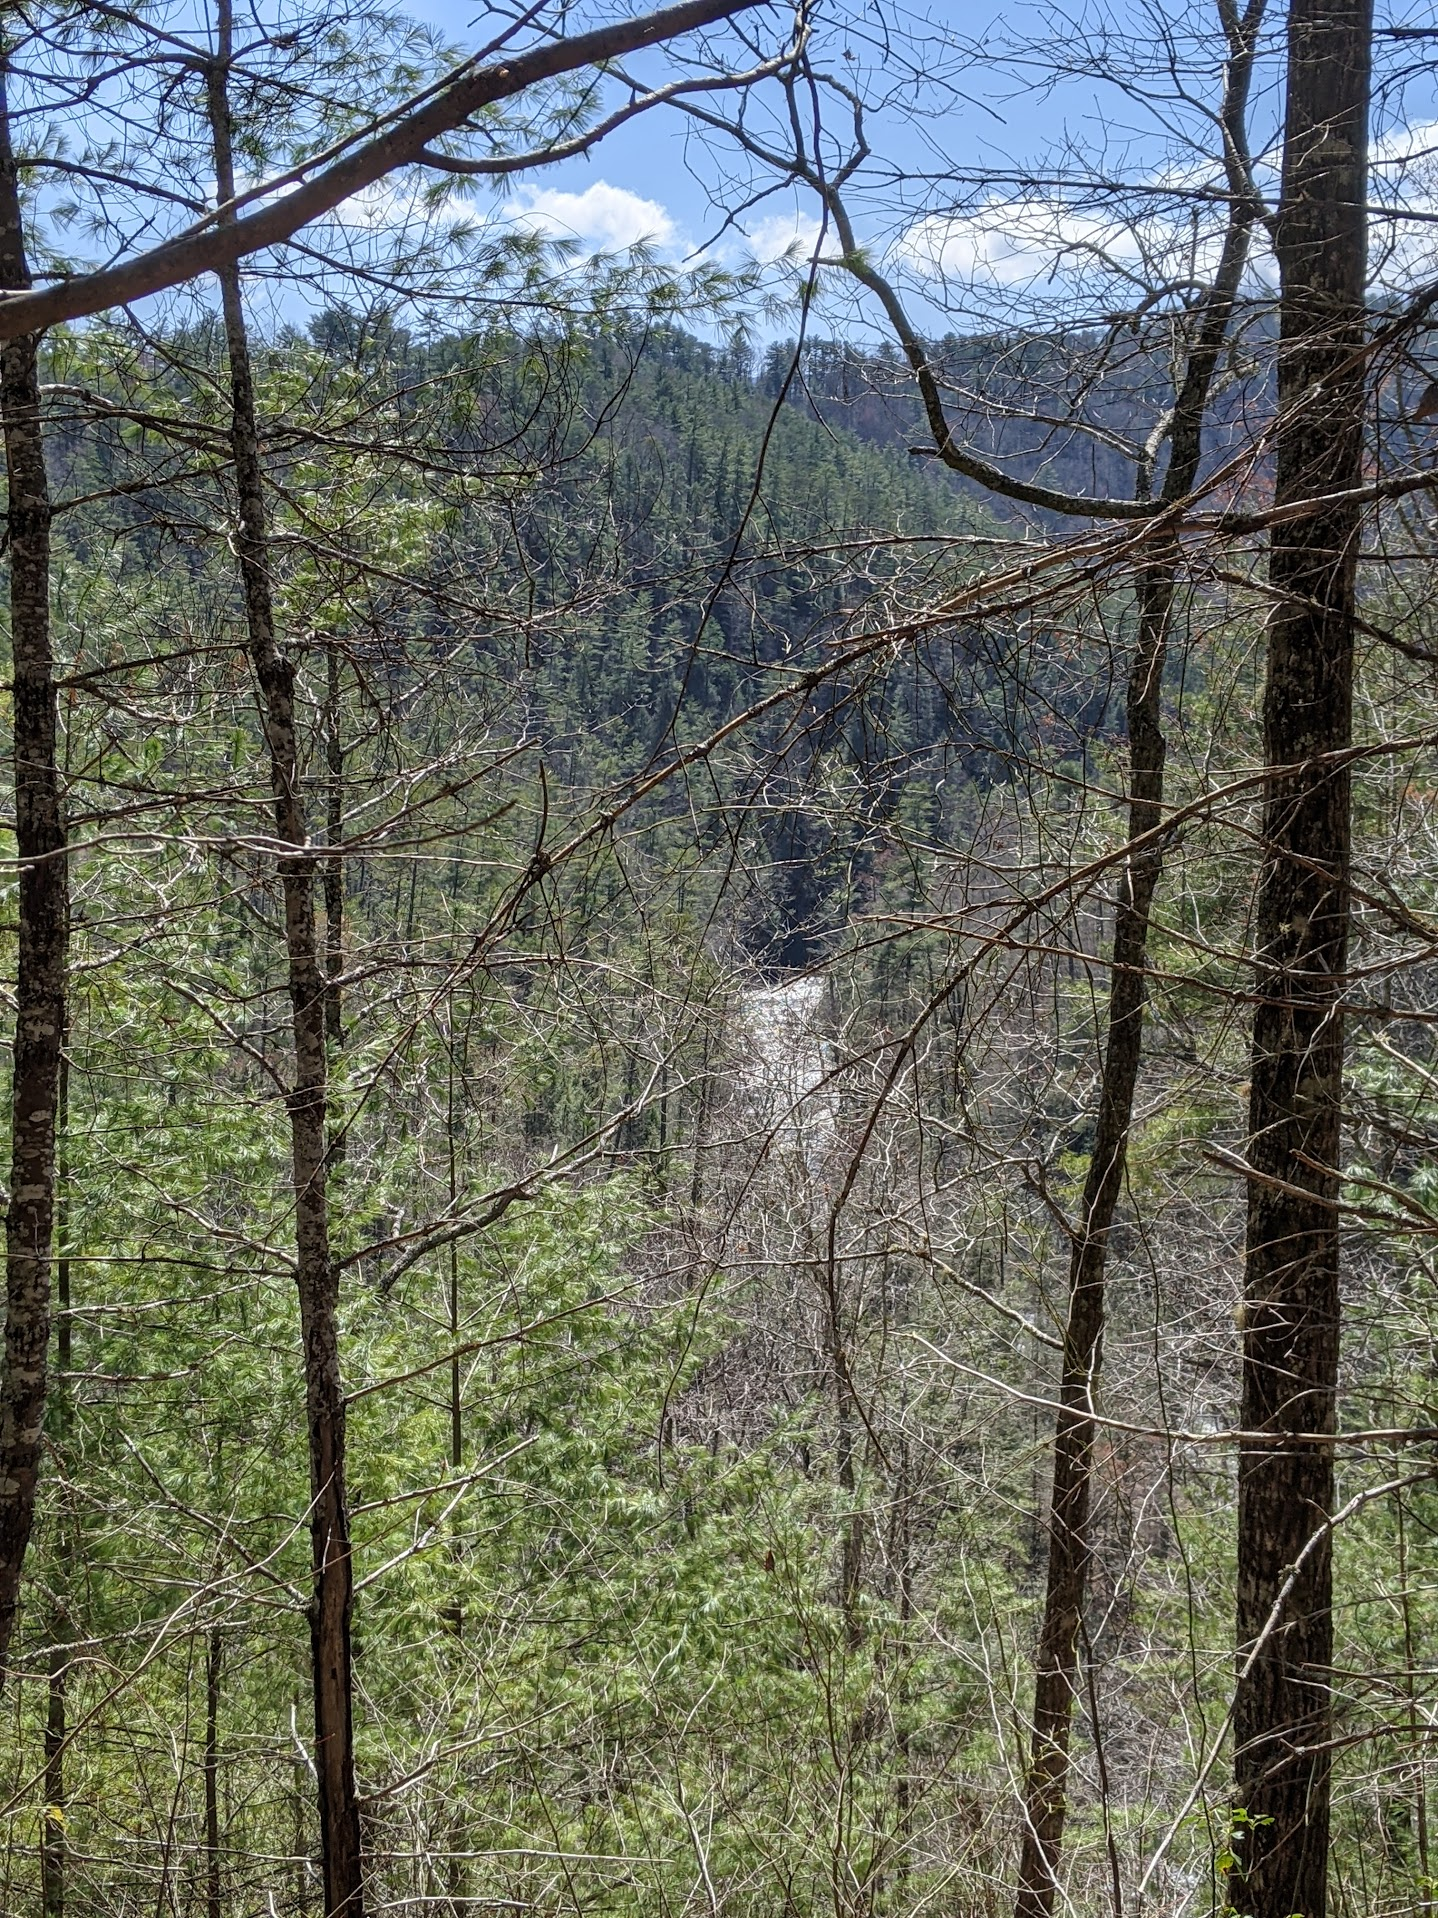
\includegraphics[width=0.9\linewidth]{/Users/joshuarosenberg/little-kids-big-adventures/img/abrams-vista} 

}

\caption{A look at Abrams Creek from the overlook along Little Bottoms trail}\label{fig:unnamed-chunk-45}
\end{figure}

From here, one of the most prominent peaks in this part of the
Smokies---Gregory Bald---is available in the distance. Thereafter, you'll head
down a fairly steep path. At **2.0 miles*, you'll return to Abrams Creek for
the first time since walking alongside it along the road near the campground!
This is - again - a great place to stop, rest, and relax---and to splash in
Abrams Creek or the small creek (Buckshank Branch) that feeds into it.

From this point onward, the trail mostly follows Abrams Creek. There are some
ups and downs, and the trail can be rocky, but the hiking is mostly free of the
ascent and descent you just completed. Around \textbf{2.5 miles}, you'll enter an
area that was once a farm.

\begin{rmdhistory}
The `bottom land' that was enriched by the run-off from and occasional
flooding of Abrams Creek was better for farming (and was---prior to the
formation of national park---farmland). This feature gives the Little
Bottoms trail its name.
\end{rmdhistory}

Finally, at \textbf{2.9 miles}, reach \emph{Backcountry Site \#17}. As we mentioned
earlier, this is a great place to rest after a strenuous hike.

\textbackslash begin\{figure\}

\{\centering \includegraphics[width=0.9\linewidth]{/Users/joshuarosenberg/little-kids-big-adventures/img/little-bottoms-site}

\}

\textbackslash caption\{Backcountry Site \#17\}\label{fig:unnamed-chunk-47}
\textbackslash end\{figure\}

From here, turn-around and return to the parking at the start, hopping along
creeks larger and smaller, perhaps a little more quickly on the way back than on
the way you headed out.

\hypertarget{nearby-13}{%
\section{Nearby}\label{nearby-13}}

\begin{itemize}
\item
  A great trip nearby Abrams Creek is \emph{Look Rock} and the \textbf{Look Rock Overlook}.
  It only adds five-ten minutes to the drive and is one of the best overlooks
  (one that is a little under-rated) in the national park. This is not strictly
  near the trailhead; instead, it's nearby the drive back, involving a turn-off
  just as you pass under the Foothills Parkway (and Chilhowee Mountain) on the
  return home from Abrams Creek. Search for ``Look Rock Tower'' or navigate to 7210
  Flats Rd., Tallassee, TN 37878 to find the parking for the overlook.
\item
  A true adventure---one that could take all day---is to continue on the Little
  Bottoms Trail past Backcountry Site \#17. Doing so leads further (2.5
  miles, one-way) to one of the most-loved waterfalls in the park, \textbf{Abrams Falls}.
  Note that the total distance of the hike from where you started (at the Abrams
  Creek Trailhead) to this waterfall would be around 11 miles, with some notable
  ascents and descents along the way. See the Abrams Falls trail entry in this
  book for another, shorter route to the Abrams Falls waterfall, if interested.
\item
  Of course, you can make a reservation to stay at either of the \textbf{backcountry
  sites} passed along this trail (Backcountry Sites \#1 and \#17). See the
  reservation system on the National Park Service's website for details;
  reservations must be made prior to the trip and are \$4 per person.
\end{itemize}

\hypertarget{middle-prong-trail}{%
\chapter{Middle Prong Trail}\label{middle-prong-trail}}

\hypertarget{trail-information-13}{%
\section{Trail Information}\label{trail-information-13}}

\hypertarget{ratings-9}{%
\subsection{Ratings}\label{ratings-9}}

\begin{tabular}{l|r|r|r|r}
\hline
Hike Name & Beauty & Accessibility & Amenities & Challenge\\
\hline
Seven Islands Island Loop & 5 & 4 & 4 & 2\\
\hline
\end{tabular}

\hypertarget{basic-characteristics-13}{%
\subsection{Basic Characteristics}\label{basic-characteristics-13}}

Location: Seven Islands State Birding Park\\
Region: The Tennessee Valley\\
Distance: 2.39 (mi.)\\
Elevation (Ascend): 191 (ft.)\\
Max. Elevation: 959 (ft.)

\hypertarget{overview-13}{%
\section{Overview}\label{overview-13}}

\hypertarget{map-13}{%
\section{Map}\label{map-13}}

\begin{figure}
\includegraphics[width=39.64in]{/Users/joshuarosenberg/little-kids-big-adventures/output/middle-prong-map} \caption{Middle Prong Trail Map}\label{fig:unnamed-chunk-49}
\end{figure}

\hypertarget{trail-description-14}{%
\section{Trail Description}\label{trail-description-14}}

\hypertarget{nearby-14}{%
\section{Nearby}\label{nearby-14}}

\hypertarget{big-creek}{%
\chapter{Big Creek}\label{big-creek}}

\hypertarget{trail-information-14}{%
\section{Trail Information}\label{trail-information-14}}

\hypertarget{ratings-10}{%
\subsection{Ratings}\label{ratings-10}}

\begin{tabular}{l|r|r|r|r}
\hline
Hike Name & Beauty & Accessibility & Amenities & Challenge\\
\hline
Big Creek & 5 & 2 & 2 & 3\\
\hline
\end{tabular}

\hypertarget{basic-characteristics-14}{%
\subsection{Basic Characteristics}\label{basic-characteristics-14}}

Location: Great Smoky Mountains National Park\\
Region: The Smokies and Beyond\\
Distance: 4.01 (mi.)\\
Elevation (Ascend): 821 (ft.)\\
Max. Elevation: 2359 (ft.)

\hypertarget{overview-14}{%
\section{Overview}\label{overview-14}}

\hypertarget{map-14}{%
\section{Map}\label{map-14}}

\begin{figure}
\includegraphics[width=39.64in]{/Users/joshuarosenberg/little-kids-big-adventures/output/big-creek-map} \caption{Seven Islands Loop Trail Map}\label{fig:unnamed-chunk-51}
\end{figure}

\hypertarget{trail-description-15}{%
\section{Trail Description}\label{trail-description-15}}

\hypertarget{nearby-15}{%
\section{Nearby}\label{nearby-15}}

\hypertarget{abrams-falls}{%
\chapter{Abrams Falls}\label{abrams-falls}}

\hypertarget{trail-information-15}{%
\section{Trail Information}\label{trail-information-15}}

\hypertarget{ratings-11}{%
\subsection{Ratings}\label{ratings-11}}

\begin{tabular}{l|r|r|r|r}
\hline
Hike Name & Beauty & Accessibility & Amenities & Challenge\\
\hline
Abrams Falls & 4 & 3 & 3 & 4\\
\hline
\end{tabular}

\hypertarget{basic-characteristics-15}{%
\subsection{Basic Characteristics}\label{basic-characteristics-15}}

Location: Great Smoky Mountains National Park\\
Region: The Smokies and Beyond\\
Distance: 4.97 (mi.)\\
Elevation (Ascend): 846 (ft.)\\
Max. Elevation: 1801 (ft.)

\hypertarget{overview-15}{%
\section{Overview}\label{overview-15}}

\hypertarget{map-15}{%
\section{Map}\label{map-15}}

\begin{figure}
\includegraphics[width=39.64in]{/Users/joshuarosenberg/little-kids-big-adventures/output/abrams-falls-map} \caption{Seven Islands Loop Trail Map}\label{fig:unnamed-chunk-53}
\end{figure}

\hypertarget{trail-description-16}{%
\section{Trail Description}\label{trail-description-16}}

\hypertarget{nearby-16}{%
\section{Nearby}\label{nearby-16}}

\hypertarget{cosby}{%
\chapter{Cosby}\label{cosby}}

\hypertarget{trail-information-16}{%
\section{Trail Information}\label{trail-information-16}}

\hypertarget{ratings-12}{%
\subsection{Ratings}\label{ratings-12}}

\begin{tabular}{l|r|r|r|r}
\hline
Hike Name & Beauty & Accessibility & Amenities & Challenge\\
\hline
Cosby Nature Trail & 4 & 3 & 4 & 2\\
\hline
\end{tabular}

\hypertarget{basic-characteristics-16}{%
\subsection{Basic Characteristics}\label{basic-characteristics-16}}

Location: Great Smoky Mountains National Park\\
Region: The Smokies and Beyond\\
Distance: 0.79 (mi.)\\
Elevation (Ascend): 124 (ft.)\\
Max. Elevation: 2390 (ft.)

\hypertarget{overview-16}{%
\section{Overview}\label{overview-16}}

\hypertarget{map-16}{%
\section{Map}\label{map-16}}

\begin{figure}
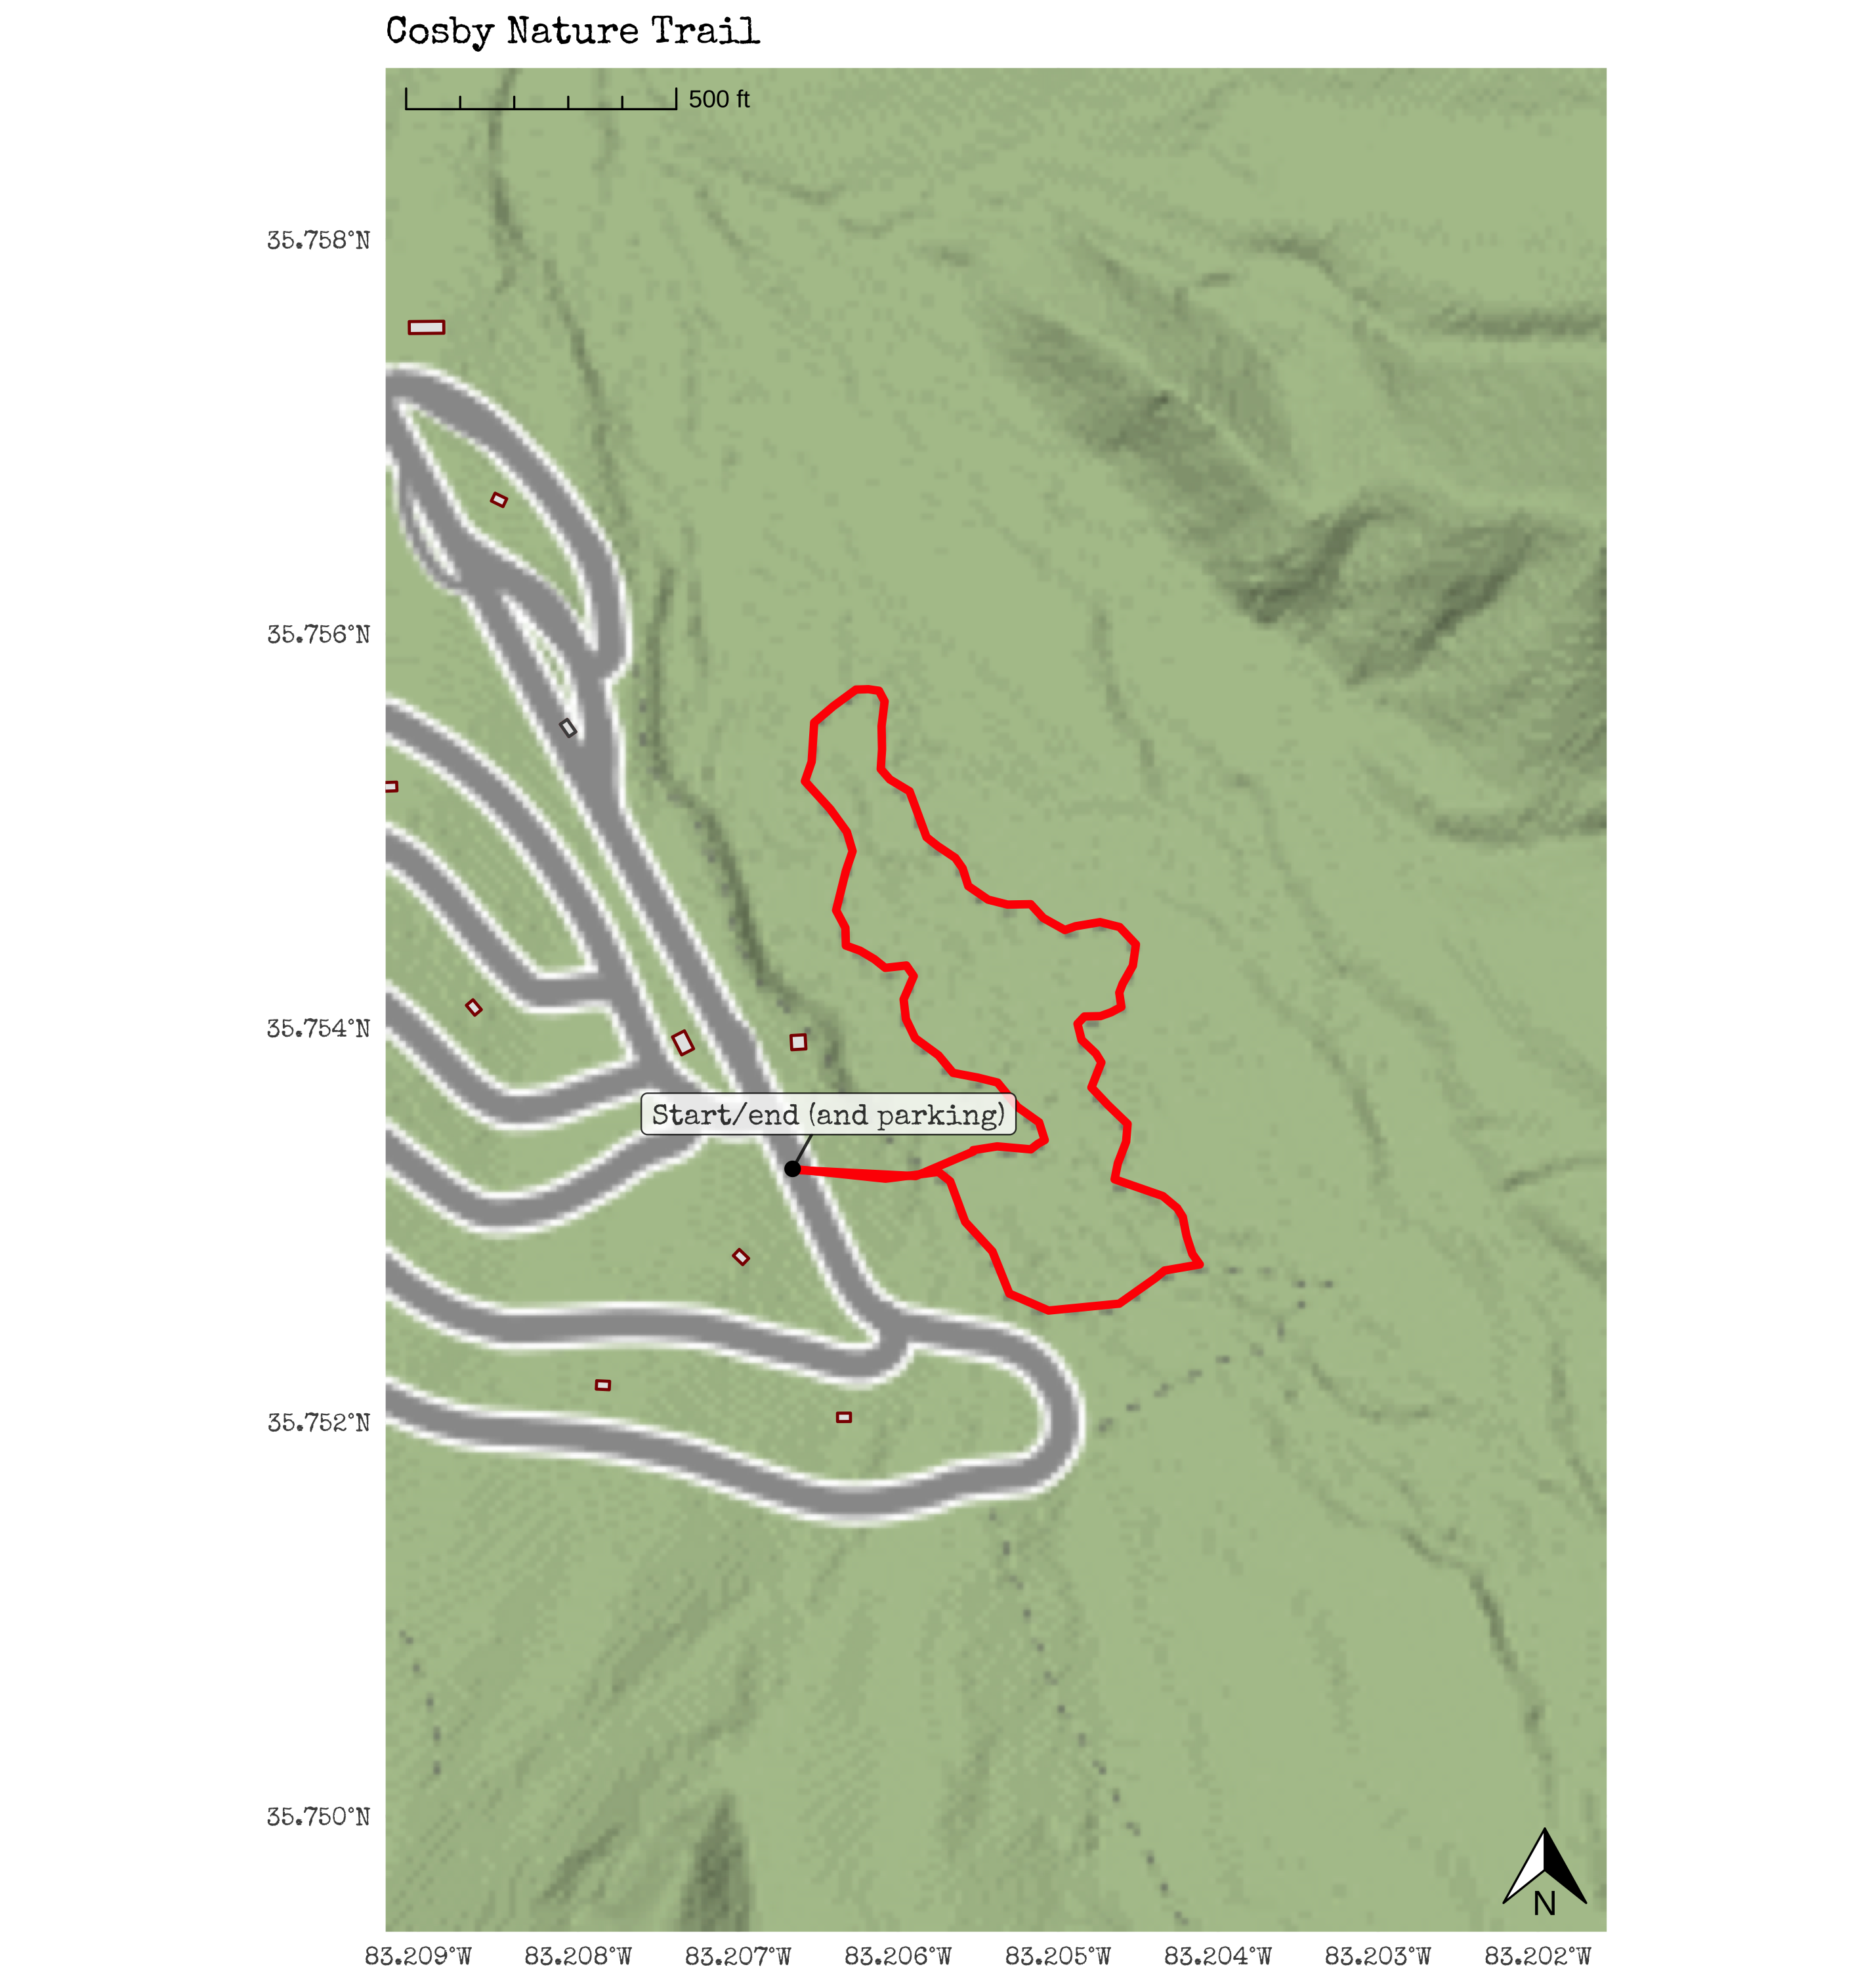
\includegraphics[width=39.64in]{/Users/joshuarosenberg/little-kids-big-adventures/output/cosby-nature-trail-map} \caption{Seven Islands Loop Trail Map}\label{fig:unnamed-chunk-55}
\end{figure}

\hypertarget{trail-description-17}{%
\section{Trail Description}\label{trail-description-17}}

\hypertarget{nearby-17}{%
\section{Nearby}\label{nearby-17}}

\hypertarget{andrews-bald}{%
\chapter{Andrews Bald}\label{andrews-bald}}

\hypertarget{trail-information-17}{%
\section{Trail Information}\label{trail-information-17}}

\hypertarget{ratings-13}{%
\subsection{Ratings}\label{ratings-13}}

\begin{tabular}{l|r|r|r|r}
\hline
Hike Name & Beauty & Accessibility & Amenities & Challenge\\
\hline
Andrews Bald & 5 & 1 & 3 & 3\\
\hline
\end{tabular}

\hypertarget{basic-characteristics-17}{%
\subsection{Basic Characteristics}\label{basic-characteristics-17}}

Location: Great Smoky Mountains National Park\\
Region: The Smokies and Beyond\\
Distance: 3.57 (mi.)\\
Elevation (Ascend): 927 (ft.)\\
Max. Elevation: 6307 (ft.)

\hypertarget{overview-17}{%
\section{Overview}\label{overview-17}}

\hypertarget{map-17}{%
\section{Map}\label{map-17}}

\begin{figure}
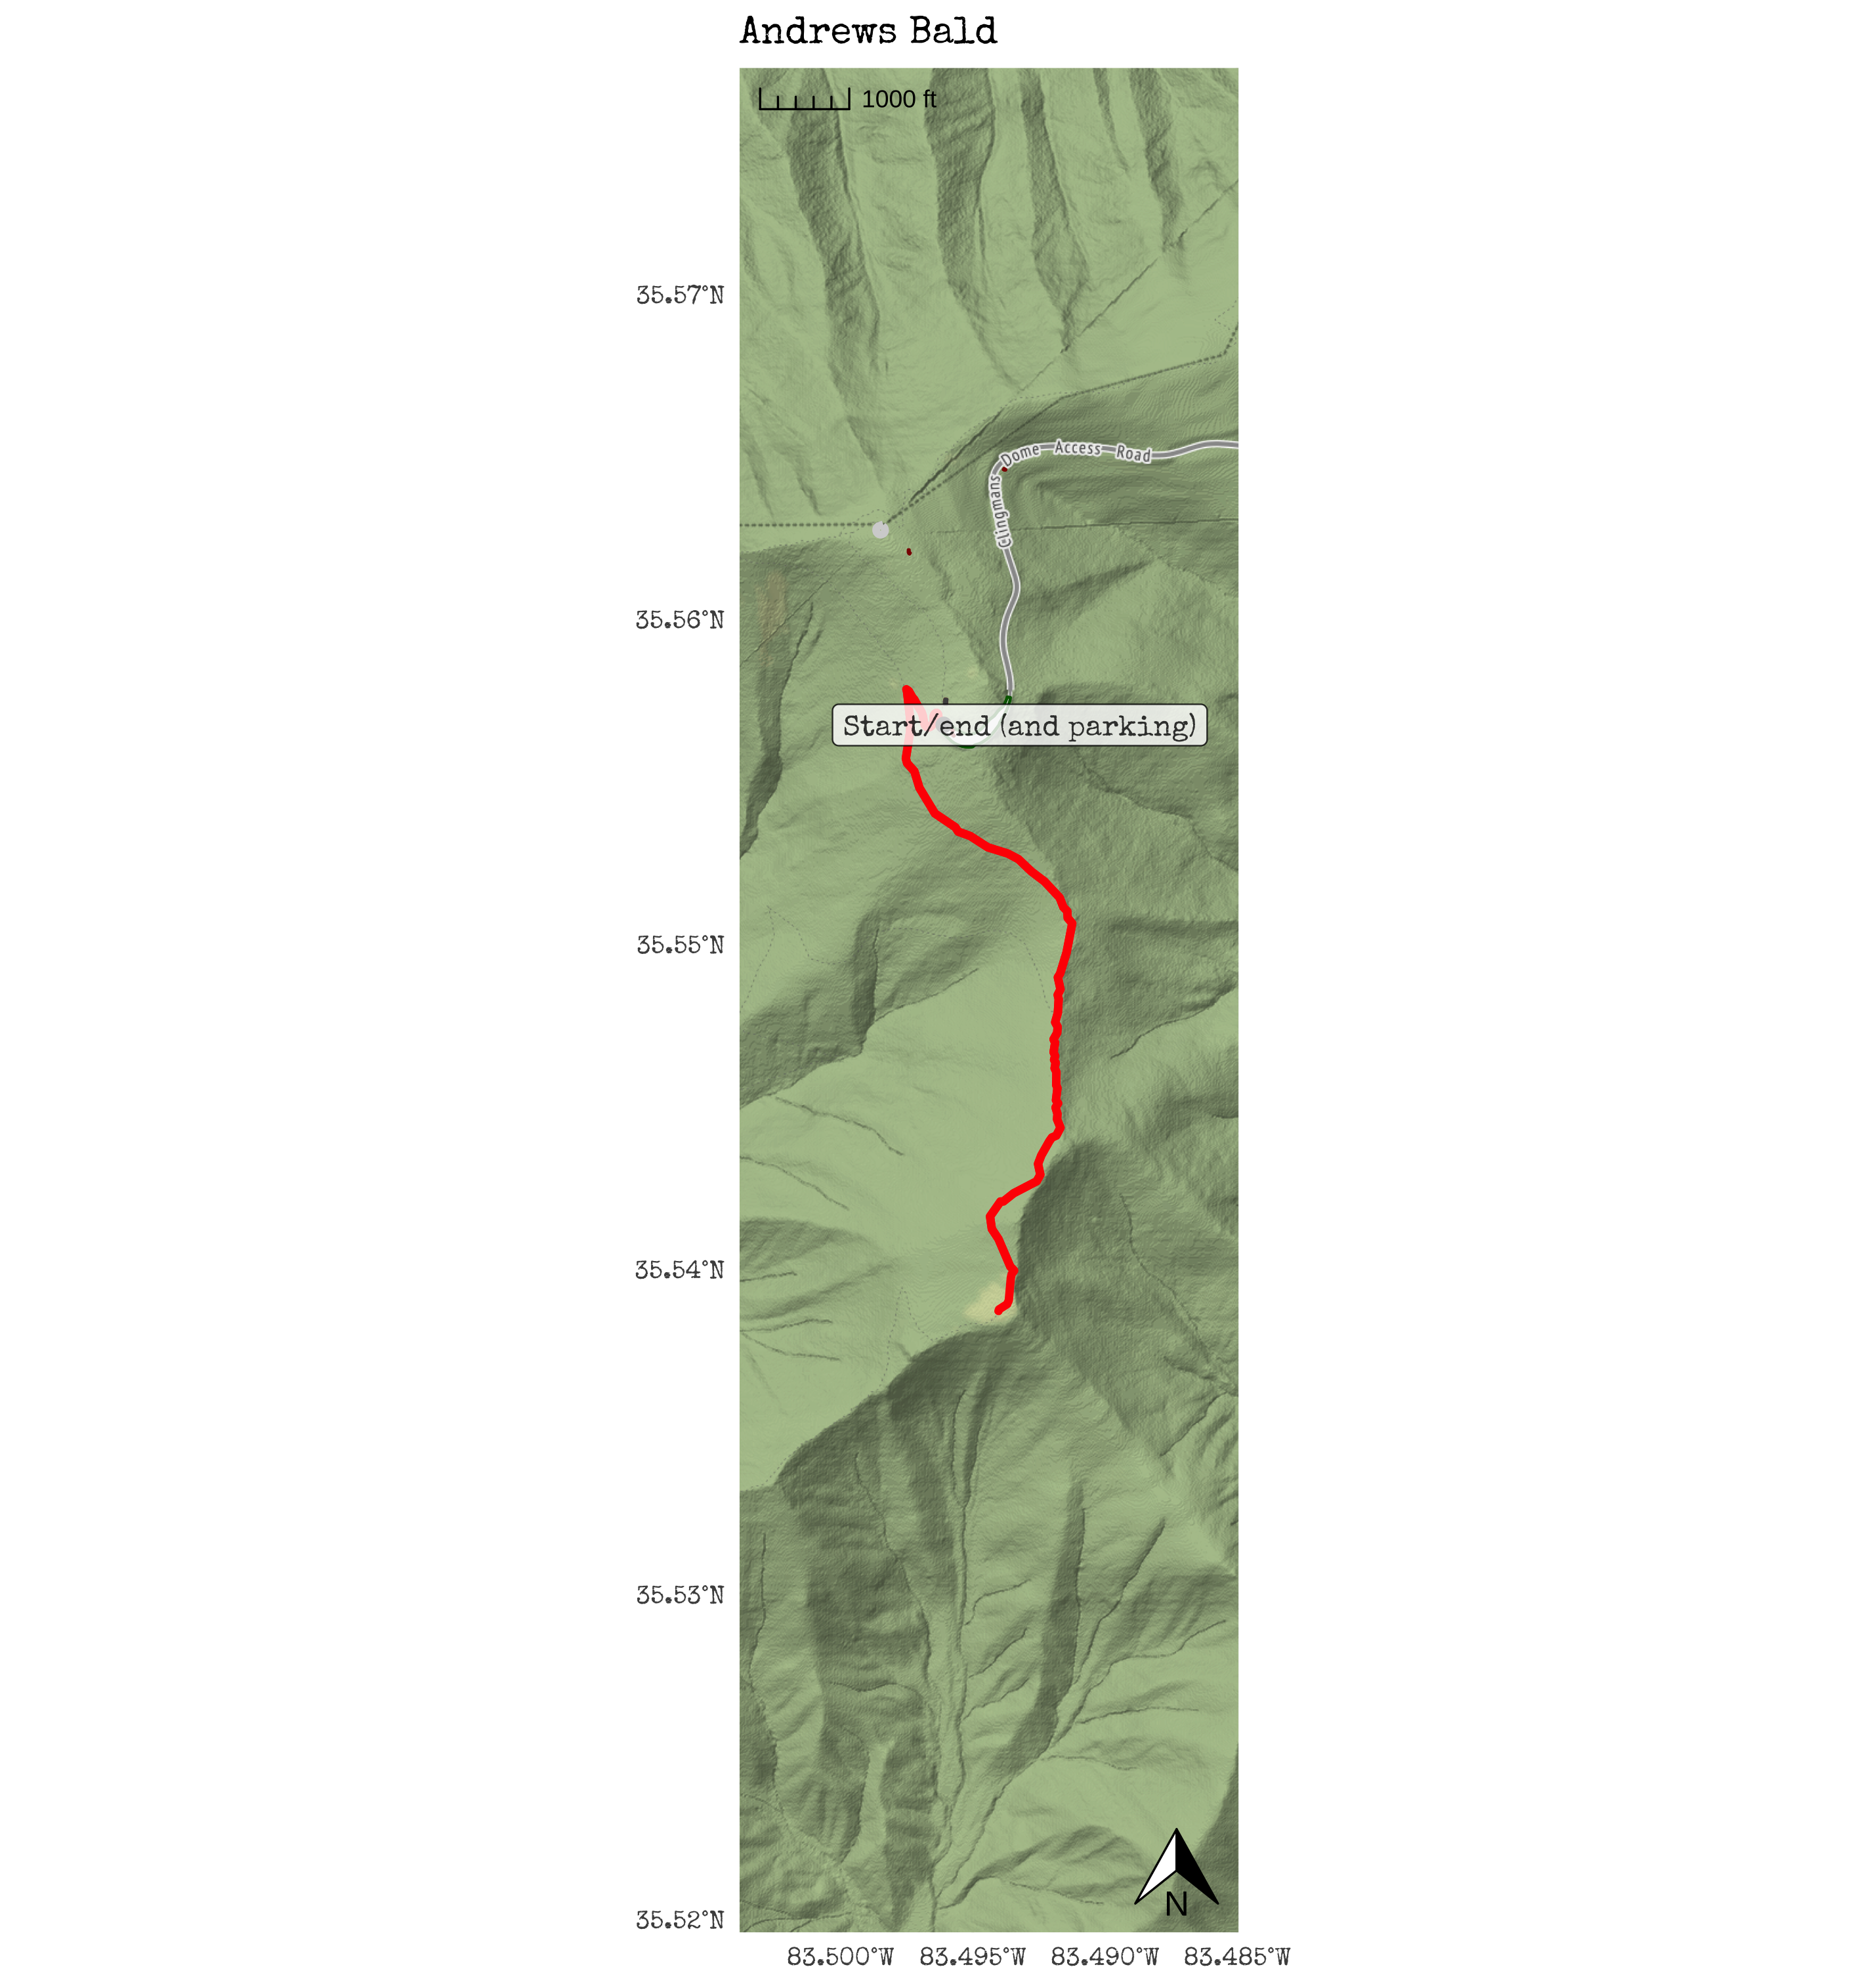
\includegraphics[width=39.64in]{/Users/joshuarosenberg/little-kids-big-adventures/output/andrews-bald-map} \caption{Seven Islands Loop Trail Map}\label{fig:unnamed-chunk-57}
\end{figure}

\hypertarget{trail-description-18}{%
\section{Trail Description}\label{trail-description-18}}

\hypertarget{nearby-18}{%
\section{Nearby}\label{nearby-18}}

\hypertarget{part-doing-more}{%
\part{Doing More}\label{part-doing-more}}

\hypertarget{top-lists}{%
\chapter{Top Five Lists}\label{top-lists}}

\hypertarget{doing-more}{%
\chapter{Doing more}\label{doing-more}}

\begin{itemize}
\tightlist
\item
  Joyce Kilmer Memorial Forest
\item
  Cherokee National Forest (portions)
\item
  (Nantahala National Forest) (portions)
\item
  (Linville Gorge)
\item
  (Mount Mitchell State Park)
\end{itemize}

\hypertarget{learning-more}{%
\chapter{Learning more}\label{learning-more}}

\begin{itemize}
\tightlist
\item
  Joyce Kilmer Memorial Forest
\item
  Cherokee National Forest (portions)
\item
  (Nantahala National Forest) (portions)
\item
  (Linville Gorge)
\item
  (Mount Mitchell State Park)
\end{itemize}

\hypertarget{giving-back}{%
\chapter{Giving back}\label{giving-back}}

\begin{itemize}
\tightlist
\item
  Joyce Kilmer Memorial Forest
\item
  Cherokee National Forest (portions)
\item
  (Nantahala National Forest) (portions)
\item
  (Linville Gorge)
\item
  (Mount Mitchell State Park)
\end{itemize}

\hypertarget{about-the-book-and-acknowledgments-and-credits}{%
\chapter*{About the Book and Acknowledgments and Credits}\label{about-the-book-and-acknowledgments-and-credits}}
\addcontentsline{toc}{chapter}{About the Book and Acknowledgments and Credits}

\hypertarget{how-this-book-was-created}{%
\section*{How this book was created}\label{how-this-book-was-created}}
\addcontentsline{toc}{section}{How this book was created}

This book is initially being written in the ``open''; this means that others can and have made suggestions that have improved it. Thank you to those who read and provided feedback on the book. We used the bookdown R package to render the book and GitHub pages to host the book.

Unless mentioned, we have taken all of the photos used in this book.

We have also created all of the maps used in this book using publicly-available data. We acknowledge those publicly-available sources next.

\hypertarget{acknowledgments}{%
\subsection*{Acknowledgments}\label{acknowledgments}}
\addcontentsline{toc}{subsection}{Acknowledgments}

Thank you to \href{https://ivelasq.rbind.io/}{Isabella Velásquez} for creating and sharing the R code to create trail maps; this code was essential to being able to create beautiful (we think!) trail maps for this book.

Thanks to \href{https://www.tylermw.com/}{Tyler Morgan-Wall}, whose \href{https://www.tylermw.com/adding-open-street-map-data-to-rayshader-maps-in-r/}{tutorial on creating trail maps} was also instrumental.

Thank you to \href{https://github.com/datalorax}{Daniel Anderson} for the basis for \href{https://github.com/datalorax/sds-r/blob/main/style.css}{the theme} for this book.

Thank you to Conor Anderson \href{https://gitlab.com/claut/man_ccia}{for the CSS code for the call-out boxes} in this text.

Thank you to Samuel Weisbrod, Aaron Rosenberg, and Kevin Lane for photos included in this book.

Thank you to Amanda Hendricks and Anthony Schmidt for trail and science-related suggestions.

\hypertarget{credits}{%
\subsection{Credits}\label{credits}}

\href{https://www.openstreetmap.org/copyright}{Open Street Map} data is used to create the trail maps.

Map tiles by Stamen Design, under CC BY 3.0. Data by OpenStreetMap, under ODbL.

  \bibliography{references.bib}

\end{document}
